%% The following is a directive for TeXShop to indicate the main file
%%!TEX root = diss.tex

\chapter{IoT Bugs}
\label{ch:bugs}

\section{Methodology}
Our goal from this study is to characterize software bugs in IoT systems. To this end, we address the following research questions in this study:
\begin{itemize}
\item {\verb|RQ1|}: What are the classes of bugs in IoT systems?
\item {\verb|RQ2|}: What are the root causes of IoT bugs?
\item {\verb|RQ3|}: What are the perceived severity and frequency of IoT bugs by real IoT developers?
\item {\verb|RQ4|}: What IoT bugs are more likely to happen together and have higher correlation?
\end{itemize}
In order to answer these questions, we conduct an empirical investigation consisting of two phases. In the first phase (RQ1), we analyze 323 issues and pull requests (PR) from open-source IoT projects. We use the findings to form the first taxonomy of bugs in IoT systems. In the second phase (RQ2), we conduct a qualitative study through (1) semi-structured interviews with IoT developers to discover new categories of bugs, (2) a survey of IoT developers to validate the findings about IoT bugs and gain new insights. All our quantitative and qualitative data is available online~\cite{repPack} 


 \begin{figure}
  \centering
   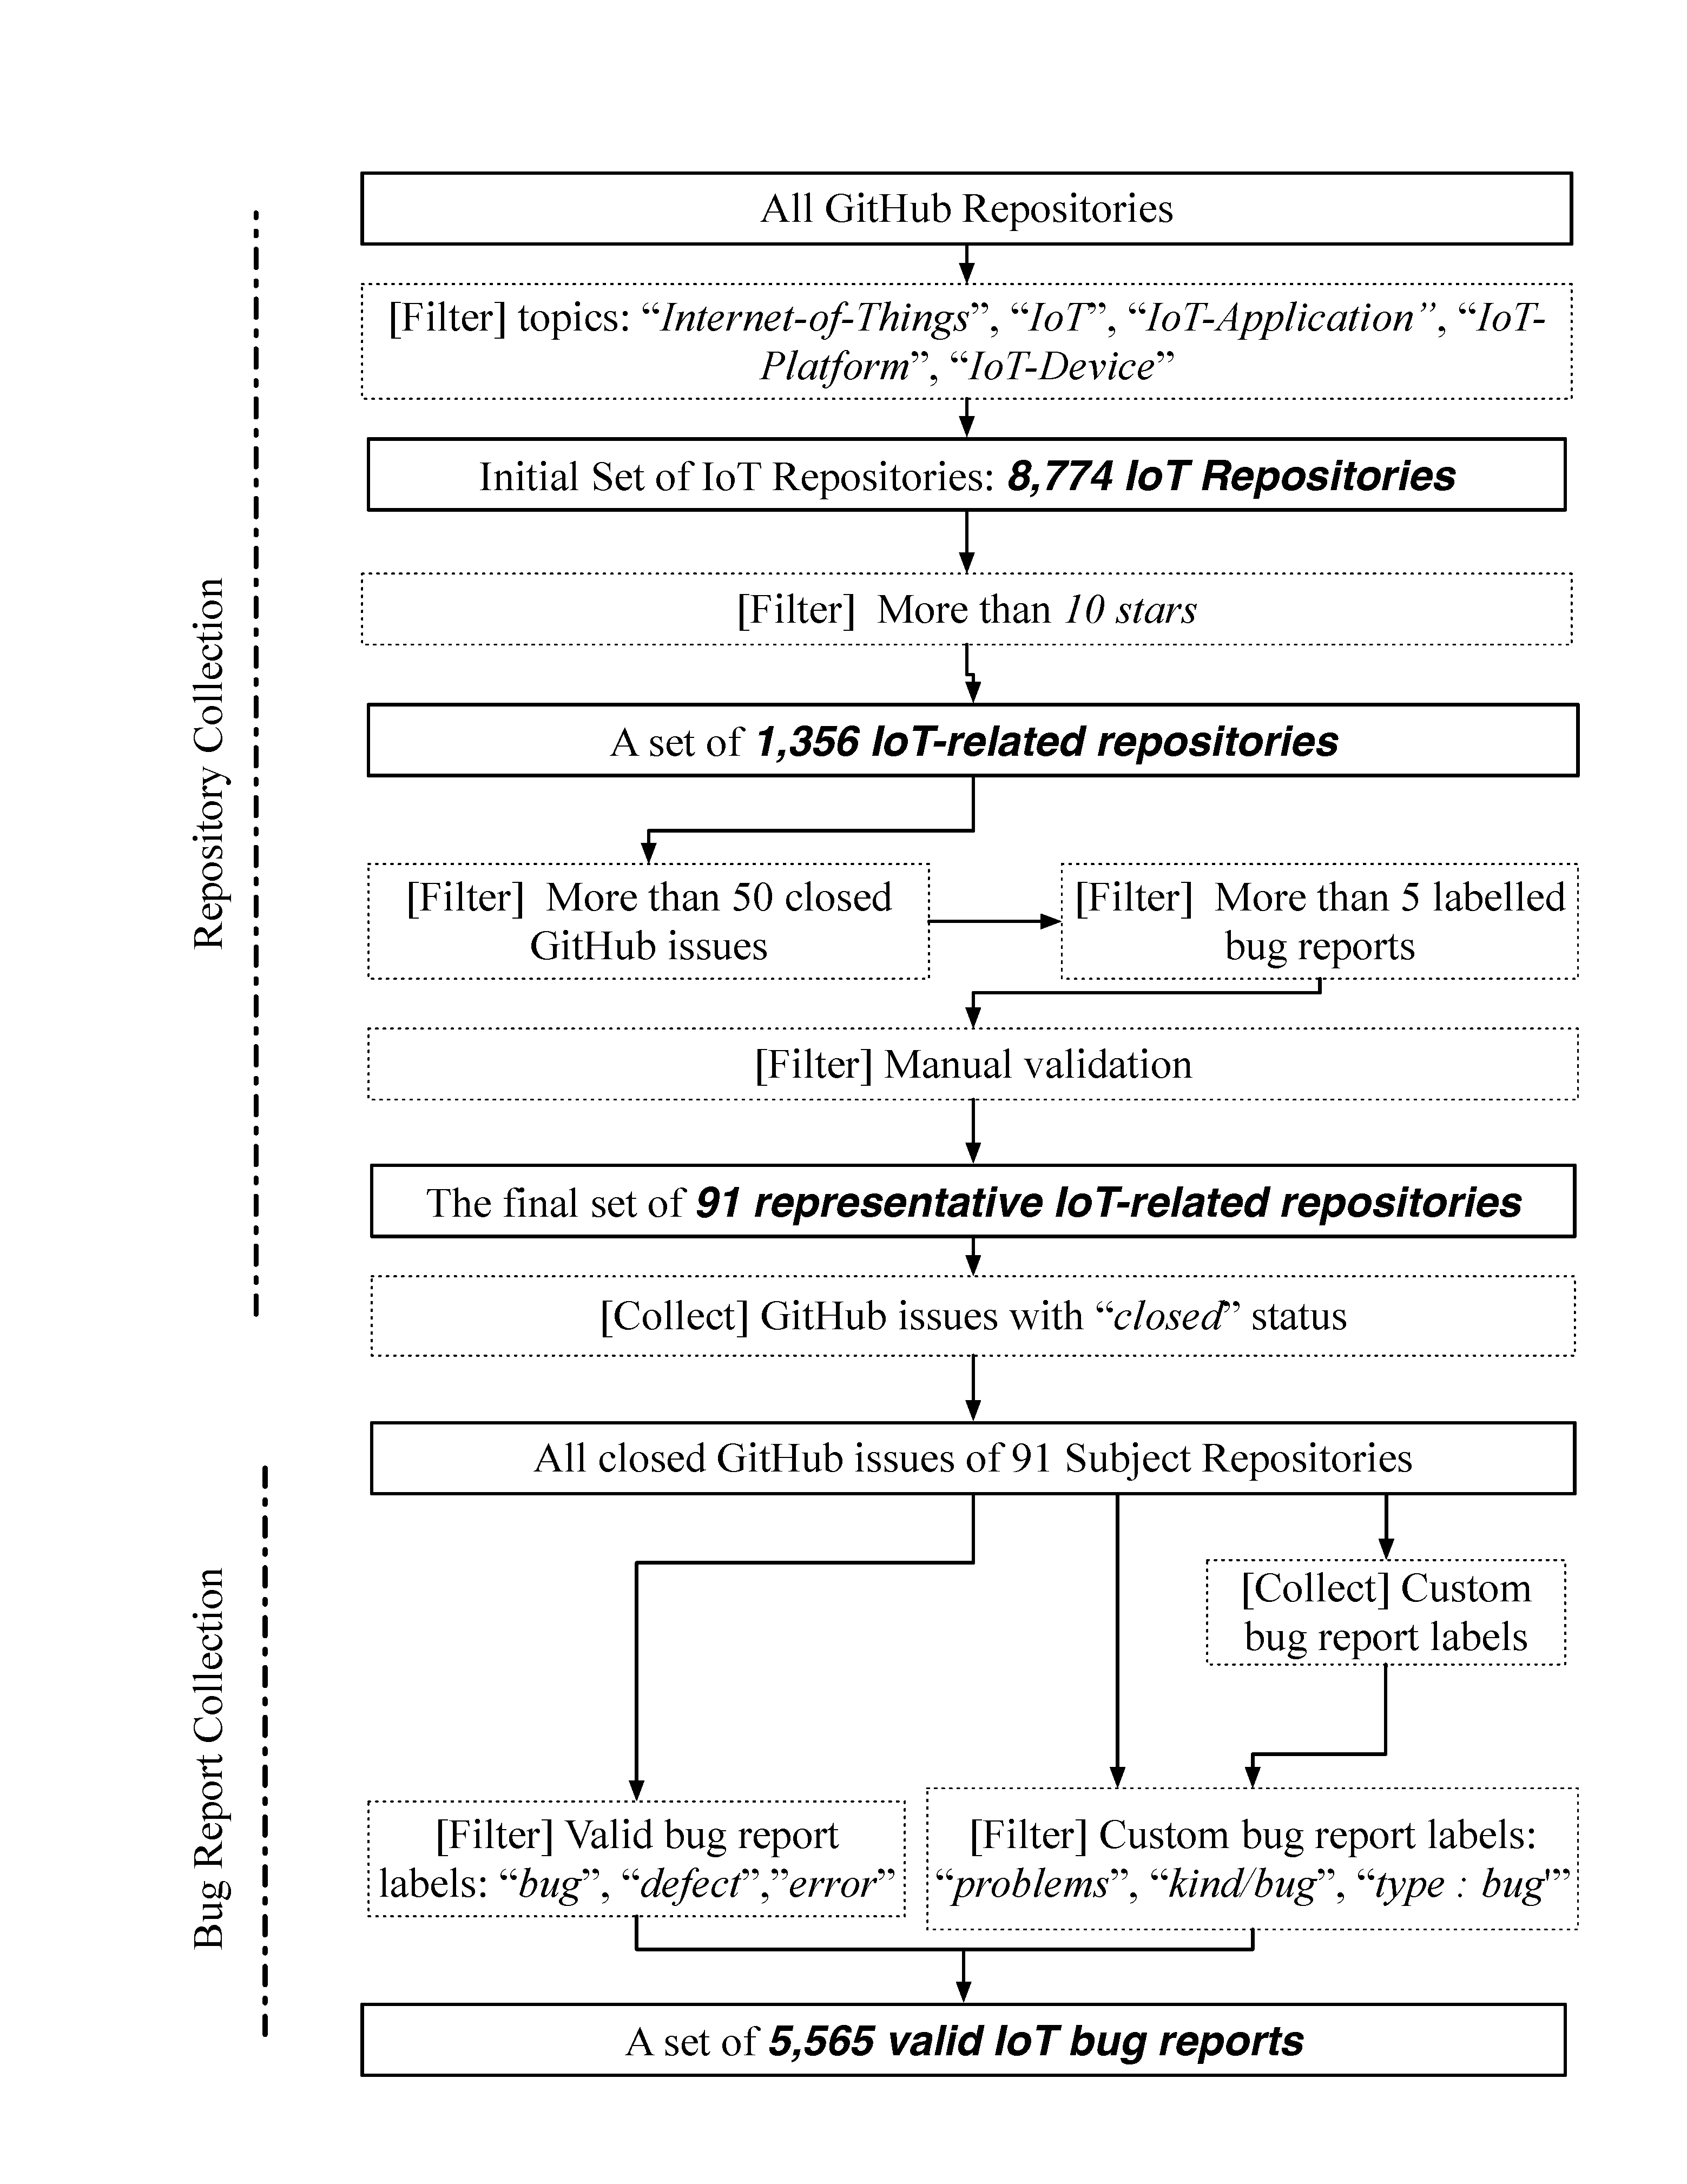
\includegraphics[width=\linewidth]{imgs/steps4repo.pdf}
  \caption{Our approach to collect subject IoT repositories and their valid bug reports.}
  \label{fig:steps4repo}
\end{figure}

\subsection{IoT Bug Categorization}
\subsubsection{Collecting bug reports} \label{bugCollection}

Figure \autoref{fig:steps4repo} shows the steps we took to find out subject IoT repositories and collect valid bug reports from them. The initial step is to find repositories that are representative of IoT projects. We employed the ``GitHub topic feature'' to find IoT-related repositories. According to GitHub's official website~\cite{gitTopic}, Topics are labels that create subject-based connections between GitHub repositories. Repository owners can use multiple tags for their repository to help users in exploring projects based on their technology, subject area, or domain.

 We searched among topics with related keywords such as "internet-of-things" and "IoT" and we added the top three topics ``IoT-application'', ``IoT-platform'', and ``IoT-device'' from the results to our list of targeted topics. Initially, we collected 8,774 repositories using these five topics in January 2020. Inspecting a random sample of 30 repositories showed that 86\% of them have less than 5 issued bug reports, while 50\% of them did not have a single bug report. A previous study~\cite{borges2018s} found that 3 out of 4 developers check the stars metric before using or contributing to a GitHub project. 
Thus, In order to reduce the number of GitHub API requests, we excluded repositories with less than 10 stars~\cite{borges2018s}, resulting in 1,356 repositories to consider.

To only consider valid bugs, we looked for issued bug reports with only ``closed'' status and with ``bug''', ``defect'', or ``error'' labels.  Moreover, to select only representative IoT repositories for our study, we manually analyzed repositories that have more than five labeled issues or more than 50 closed issues based on the information in their readme page, issued bug reports, and their website (when available). We then excluded projects that were not representative of IoT systems such as user interface, documentation, or outdated repositories. Our final project list contained 91 open source IoT repositories to analyze. For five repositories that use custom labels (e.g., ``problems'', ``kind/bug'', ``type : bug''), we manually added their labels to our search keywords. In the end, we collected \emph{5,565 bug reports} from the 91 IoT repositories.

Figure \autoref{fig:repodemog} shows the demographics of our subject repositories. The selected IoT repositories together cover all the layers of the IoT systems' architecture depicted in \autoref{fig:arch}. The most popular programming languages among the subject repositories are Python (21\%), Java (18\%), JavaScript (17\%), C (13\%), and C++ (13\%). A few of them use other programming languages such as Go, Ruby, and C\#. The selected repositories are also diverse in terms of the number of stars and forks they have. In February of 2020, 32\% of our subject GitHub repositories had more than 500 stars, 40\% between 50 to 500 stars, and 28\% between 10 to 50 stars.


 \begin{figure}
  \centering
   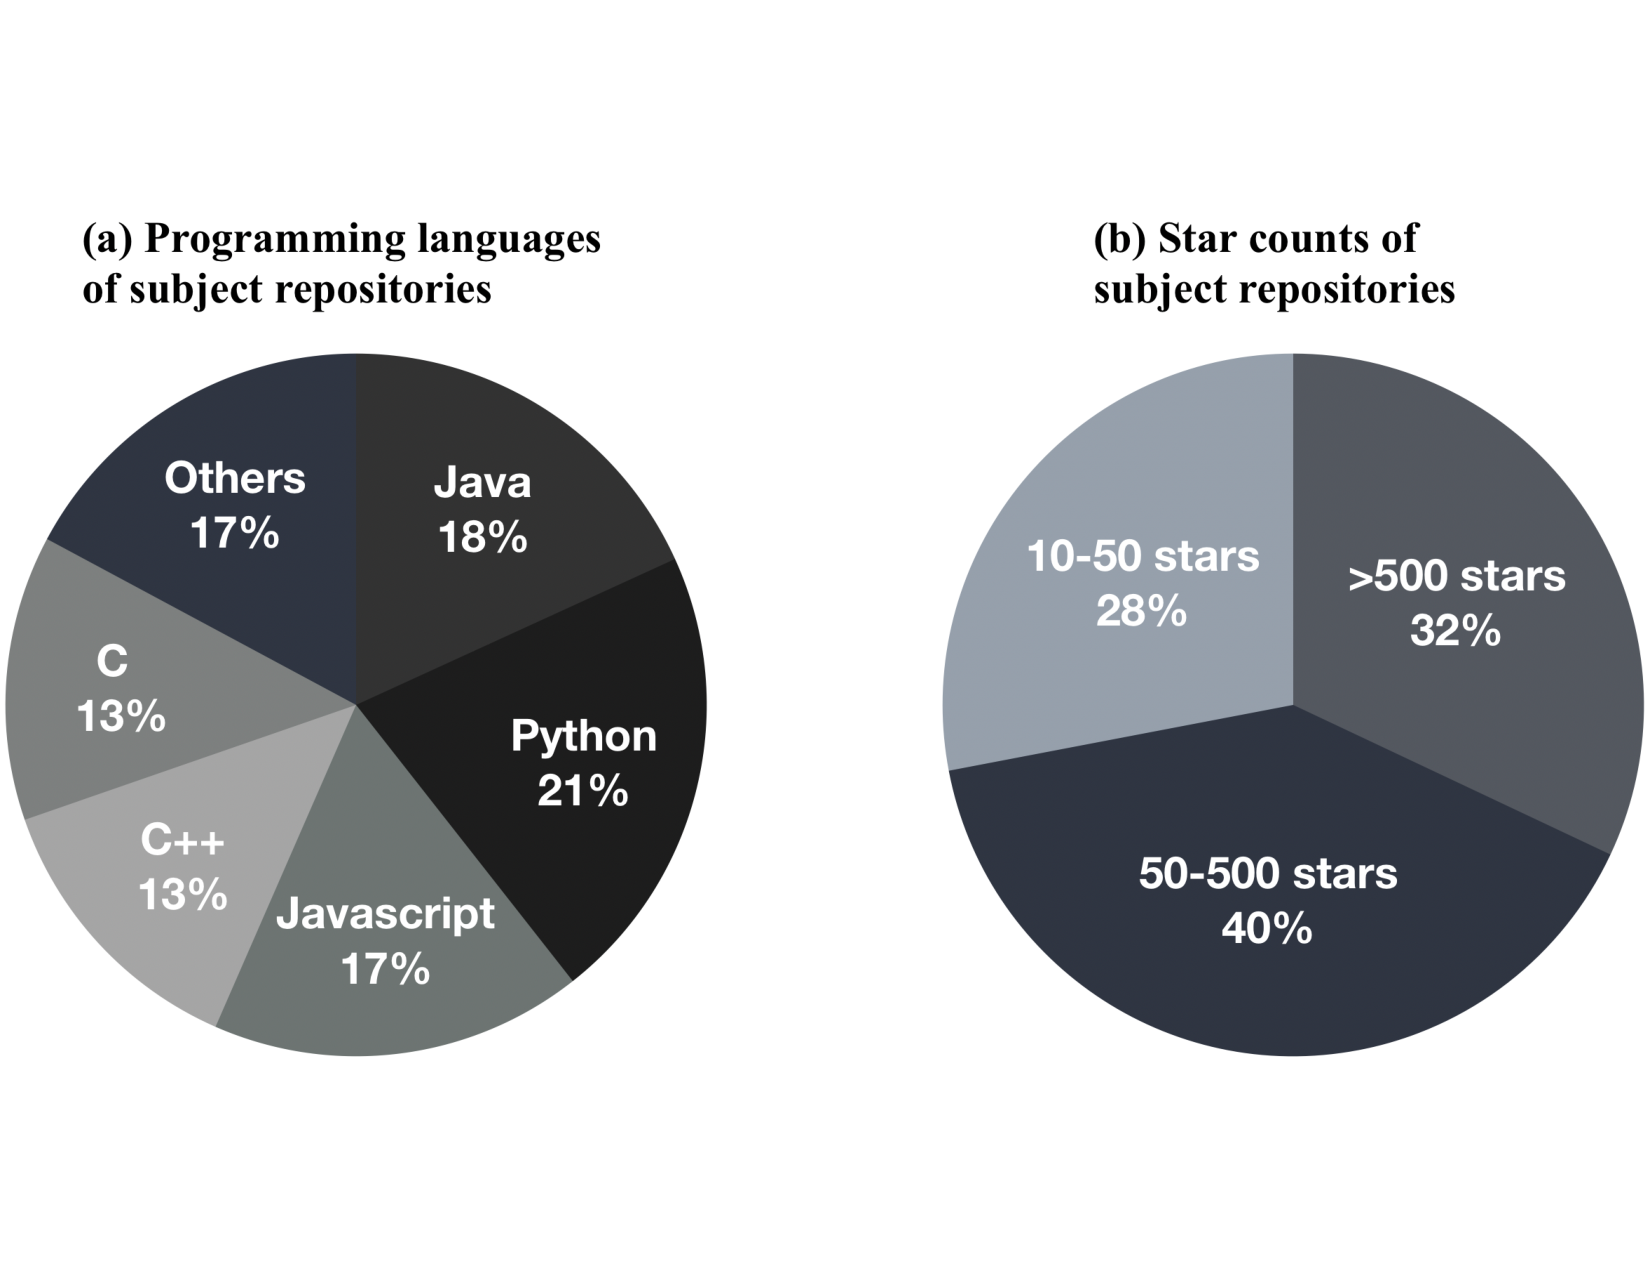
\includegraphics[width=\linewidth]{imgs/repodemog}
  \caption{(a) Programming languages of subject repositories and (b) their star count.}
  \label{fig:repodemog}
\end{figure}


\subsubsection{Labeling} 
Figure \autoref{fig:labeling} shows the steps we took to label bug reports. For each bug report in our dataset, we created a JSON object containing failure(s), cause(s) of the failure, and location(s) of the faulty code. Failure refers to any observable unexpected behavior of the system that is against the correct functionality of that system~\cite{bugCharOpenSoftware,failureDefinition}. To explore the causes of the failure, we did RCA on each bug report using the \emph{five whys technique}~\cite{serrat2017five}. Based on this technique, multiple causes can contribute together or at different levels to a visible failure in the system. Following this approach, we started from the failure and repeatedly asked ``why'' until we reached the root cause of the problem. In the case of software failures, root causes are often developers' faults in the design or implementation of the IoT system. To label the location(s) of faults, we used the architecture defined in Chapter \ref{ch:background} as our reference. 

Bug reports were manually labeled by the author(s) individually following the open coding procedure~\cite{qualitativeStudySE}. We followed an iterative process for labeling where in each iteration, we randomly sampled new instances from the collected bug reports and labeled them. After each labeling iteration, all potential conflicts in labels between the author(s) were resolved. We continued this process until bug categories reached a state of saturation where no new category appeared~\cite{dataSaturationFusch}. 

We also flagged and discarded issues and PRs that could not represent a bug or a bug-fix such as enhancements or how-to-use questions. We examined the entire discussion among developers, as well as the fix commit data (e.g. the commit message and the code diff) to label each bug report. At the end, we labeled \emph{323 bug reports}.

 \begin{figure}
  \centering
   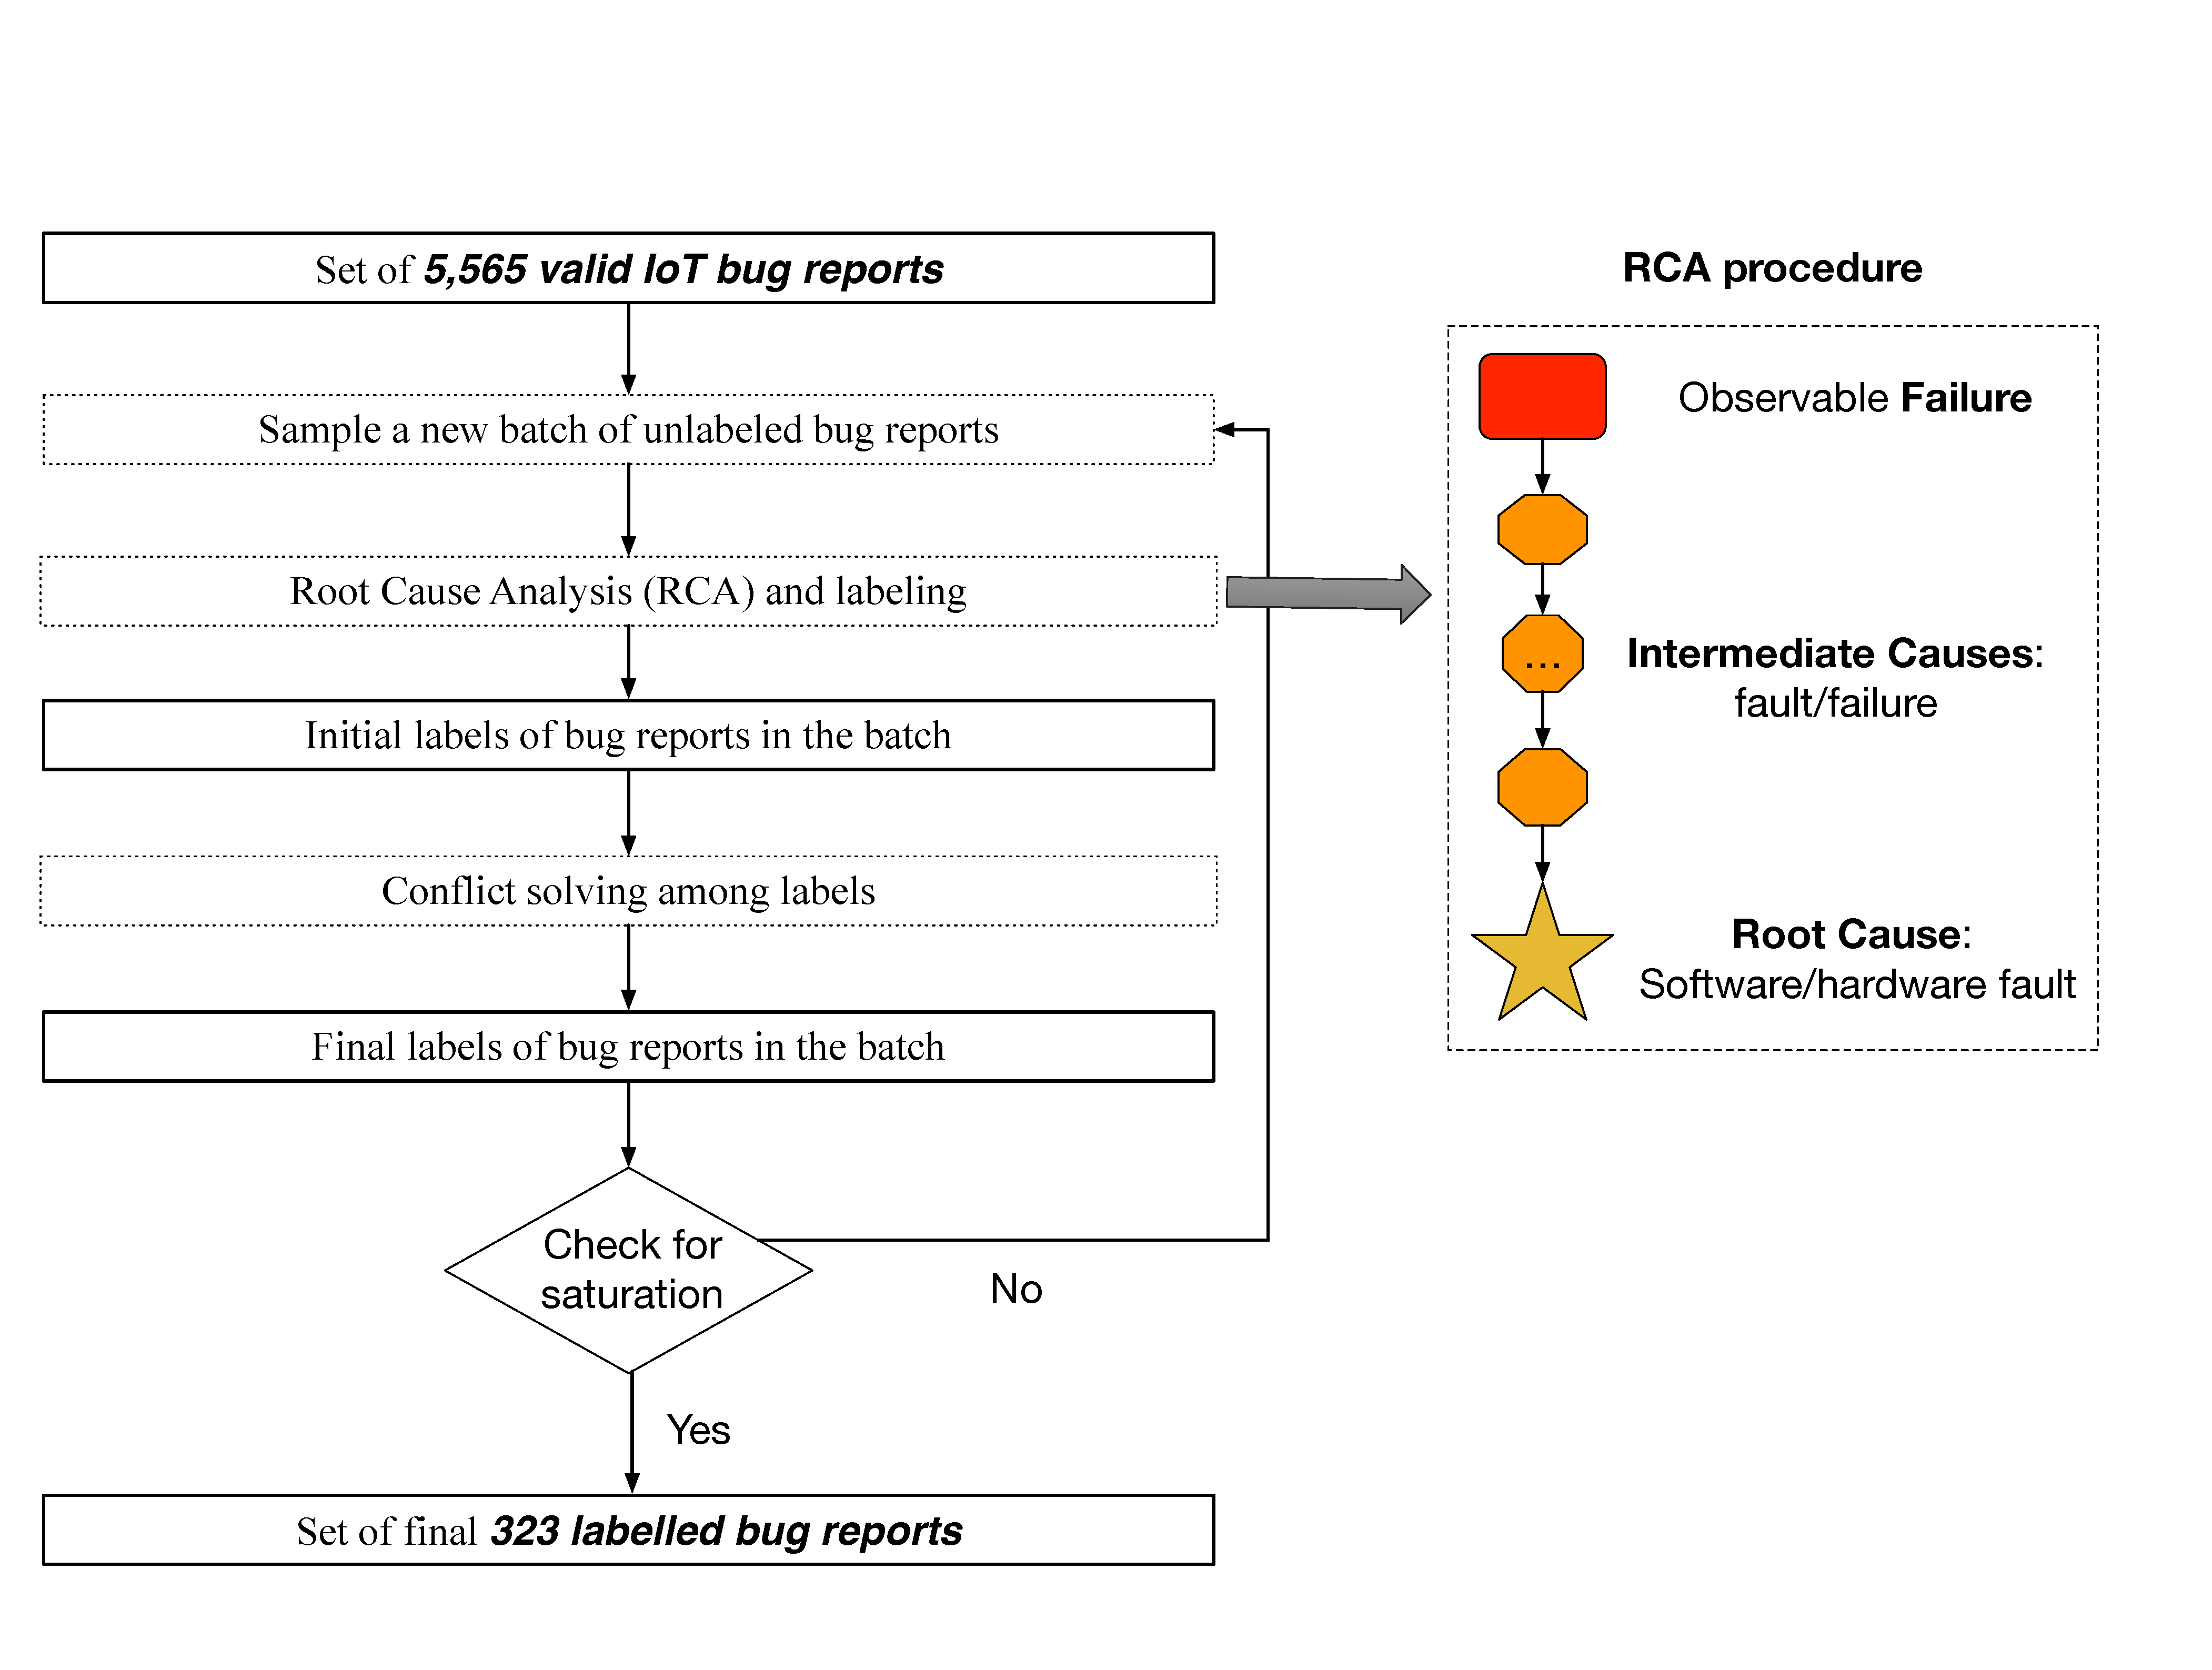
\includegraphics[width=\linewidth]{imgs/labeling}
  \caption{(a) Programming languages of subject repositories and (b) their star count.}
  \label{fig:labeling}
\end{figure}

\begin{table}[htbp]
\caption{Interview Participants}
\resizebox{\linewidth}{!}{%
\begin{tabular}{c l l l r r}
\hline
\textbf{ID}& \textbf{Role }&\textbf{IoT Systems Type}& \textbf{Projects Domain}  & \textbf{Dev Exp (yr)} & \textbf{IoT Dev Exp (yr)}  \\
\hline
P1 &  Software and hardware lead & Full-stack & Smart home  & 13  & 7   \\
P2 & Hardware lead & Hardware & Education& 15  & 5    \\
P3 & Software dev & Full-stack & Smart home & 5  & 4   \\
P4 & Software dev & Middleware & Smart city & 3  & 3    \\
P5 & Software lead & Full-stack & Smart home & 20  & 17   \\
P6 & Software dev  & Cloud &  Not domain-specific & 10  & 3 \\
P7 & Software and hardware dev & Full-stack & Smart home & 20  & 3   \\
P8 & Software lead  & Full-stack & Smart home & 11  & 4  \\
P9 & Software lead  & Cloud & Not domain-specific & 20  & 12  \\
\hline
\end{tabular} }
\label{tab1}
\end{table}

\subsection{Interviews} \label{interviews4Bug}
 While manual analysis of bug reports and developers' discussions provided useful insights into the characteristics of IoT development, there was still a possibility that our bug categories are not generalizable. To mitigate this issue, we conducted semi-structured interviews with IoT developers to reveal new bug categories to complement and validate our results. 

\textbf{Participants} 

To collect interview participants, we employed GitHub as it provides a diverse pool of developers and their contributions to different projects.

To collect candidate interview participants, we followed the steps shown in figure~\autoref{fig:candidates}. We used the 1,356 IoT repositories we collected in section~\autoref{ bugCollection}, as the IoT projects with more than 10 stars, to sample interview participants. After collecting all the 11,129 contributors to these 1356 repositories, we removed duplicate contributors, resulting in 6,878 contributors. Duplicate contributors are the IoT developers involved in more than one repository from the set of subject repositories and thus appeared more than once in our initial dataset. The next step is to find the valid email addresses of these unique contributors.


GitHub API does not provide the email addresses of the developers directly. We searched through the information returned by GitHub public API from the requests regarding contributors' commits to extract their email addresses. This was the only way we could find to extract the email addresses of contributors to IoT repositories.  A manual run of this method showed that the email addresses of a handful of the contributors are unavailable or invalid. First of all, we removed the contributors that their email address has not appeared in any of the GitHub API's responses since our goal was to contact developers only via their email addresses. Moreover, we removed the contributors that their email address contains the string "no-reply" and its invariants. After all the filtering, we could obtain the valid email addresses of 1,847 unique contributors to popular IoT repositories.

For interviews, we only added the top three contributors to the set of candidate interviewers. We used purposive sampling~\cite{sampling2007} to recruit developers with adequate experience in developing IoT systems.  

We contacted candidates through emails and conducted interviews until we reached data saturation, where we had sufficient data to replicate the study and further data collection is unnecessary~\cite{dataSaturationFusch}. We relied on this widely-applied methodological principle to decide when to stop interviewing~\cite{saturationMorse,saturationGuest} as it is also used in other qualitative studies in software engineering~\cite{tweeter2014, aniche2018modern}. We interviewed people with different development backgrounds and experiences before deciding about the data saturation to consider variability in experimental results across different populations~\cite{henrich2010weirdest}. 


 Table \ref{tab1} presents all nine interview participant's experience and field of expertise in IoT development. For a high-level picture of their general development background, the lowest value is three years and the highest value is 20 years (avg=13, sdv=6.4). In terms of IoT development experience, the lowest value is three years and the highest value is 17 years (avg=6.4, sdv=4.6). Participants' IoT development experience covers all sections of IoT systems spanning from hardware to middleware, cloud, and end-applications. In addition, their projects cover a variety of domains such as smart home and Industrial IoT (IIoT). 

\afterpage{%
 \begin{figure}
  \centering
   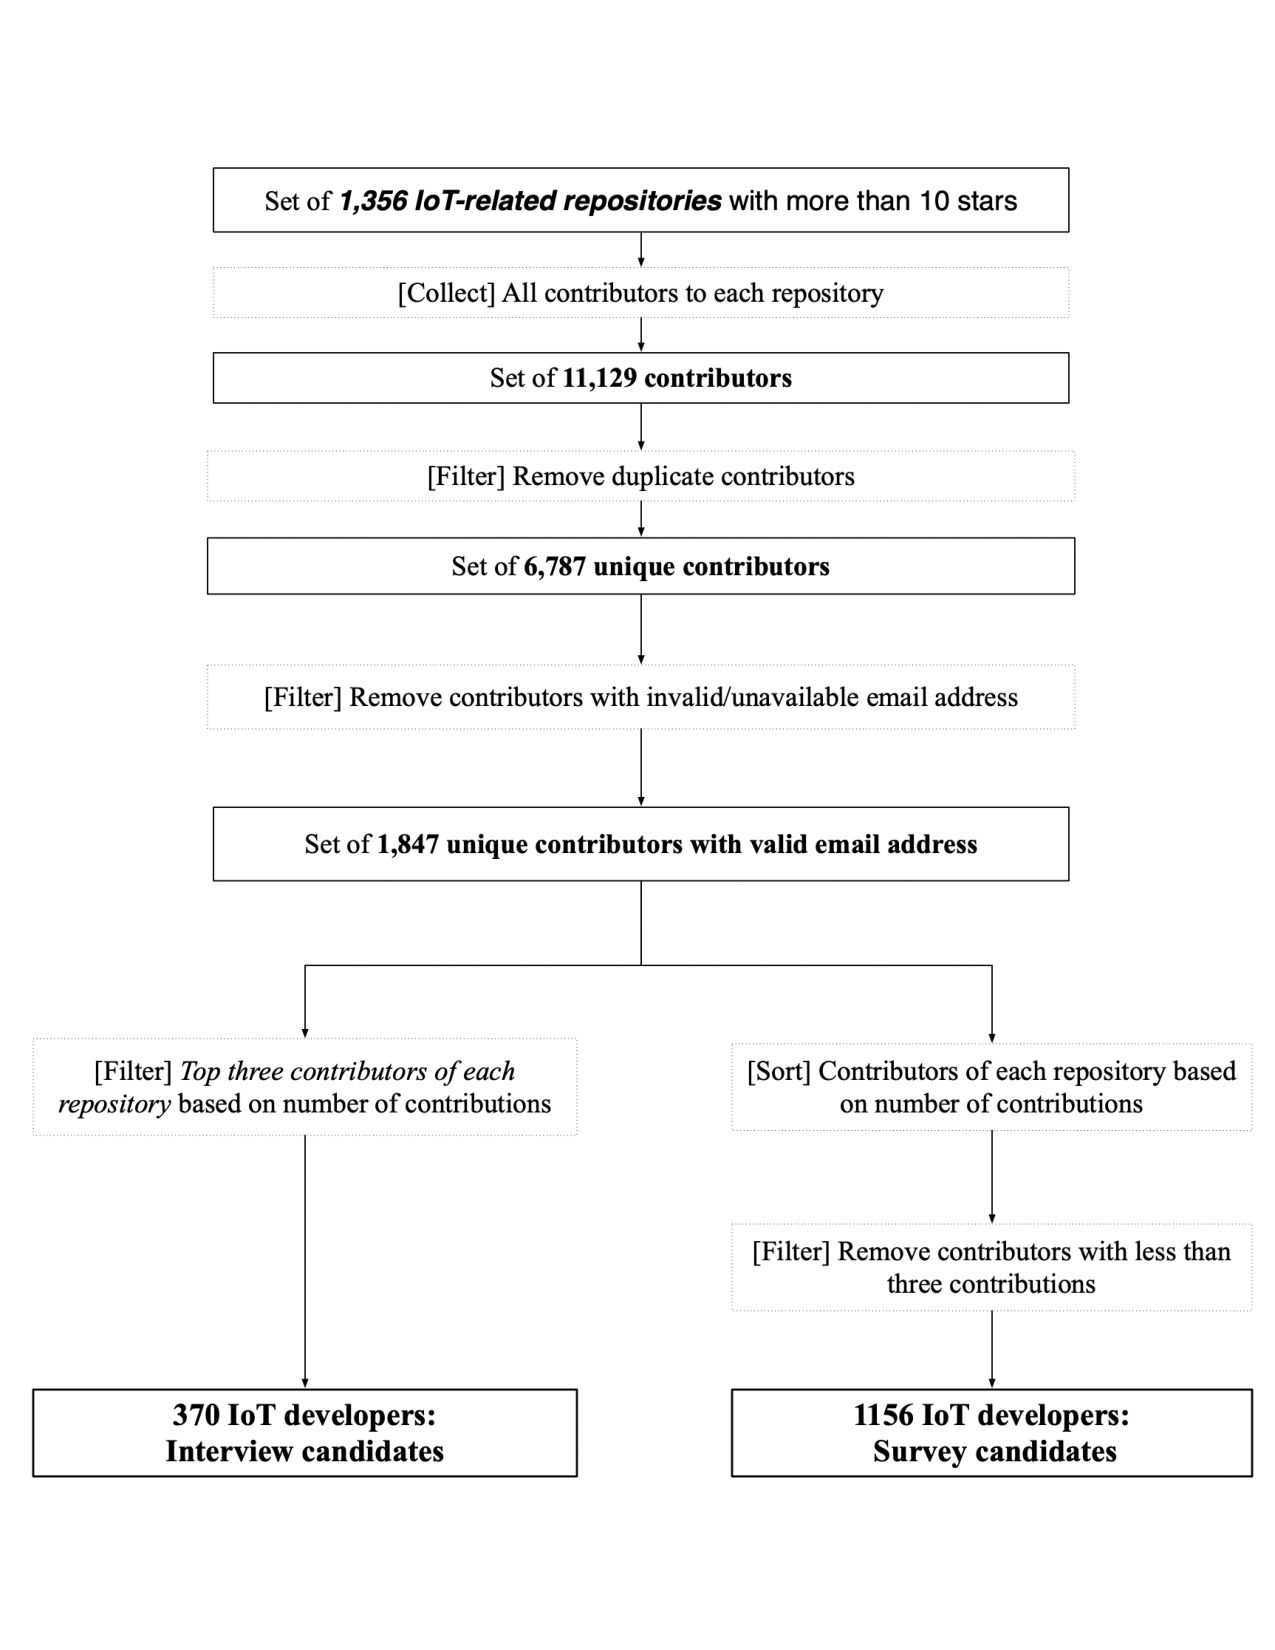
\includegraphics[width=\linewidth]{imgs/candidates.pdf}
  \caption{Our methodology for finding candidates for interviews and survey.}
  \label{fig:candidates}
\end{figure}
\clearpage
}

\textbf{Protocol} \label{interviewProtocol}
Since our goal for conducting interviews was to be open to new data, and we did not have the definitive structure of bug categories, we conducted interviews following a semi-structured approach. Interviews started with some questions about participants' IoT development background and their field of expertise in IoT. This information could help us improvising insightful questions during the technical section of the interviews. The technical section had a combination of both open-ended and specific questions about different categories of bugs and challenges in IoT development. Our strategy was to start with open-ended questions to avoid biasing participants toward our findings, and then we gradually shifted to more structured and predefined questions during the interview process.  With participants' consent, we recorded the audio and video of all the interviews for later analysis. All the interviews were conducted remotely through Zoom. Interviews took around 43 minutes on average ranging from 31--70 minutes. We used Descript, an automated speech detection tool, to generate transcribes of the interviews and we did manual corrections afterward in case of any mistakes in the automatically generated transcripts.

\textbf{Analysis} \label{interviewAnalysis}
As the primary objective of this study is to generate theories from the experiences of IoT practitioners instead of using pre-conceived theories, we followed the grounded theory methodology~\cite{grounded2007} to ensure the quality of the generated theory. Our analysis steps consist of iteratively (i) collecting qualitative data from the interviews (ii)  analyzing the interview transcript line by line and assigning labels (tags) to distinct units of meanings, and (iii) identifying emerging categories and relating categories to their subcategories while continuously comparing all the previously analyzed data with the emerging theories. These steps were repeated for each interview. On average, we extracted 18 tags per interview. Potential conflicts in the labels were resolved after each iteration by the authors. 

\subsection{Validation Survey} \label{survey4bug}
In order to make sure that our findings are generalizable, comprehensive, and representative, we involved more IoT developers through an online survey. 

\textbf{Participants} 
Figure~\autoref{fig:candidates} shows how we collected the survey participant candidates. Firstly, we sorted the collected unique contributors with valid email addresses based on the number of contributions they had to the 1,356 subject IoT projects. After removing the contributors with less than three contributions, we started to send out our survey to the resulting candidate participants until we reached saturation in our results. We gave higher priority to the developers with more contributions by sending our survey first to the developers with higher contributions.

We also sent out our survey to the IoT developer groups in social media platforms such as Linkedin and Facebook, and online forums. Our survey was online between 19 July and 19 August 2020. The survey, as distributed to participants, is available in our artifact package~\cite{repPack}.
 \begin{figure}
  \centering
   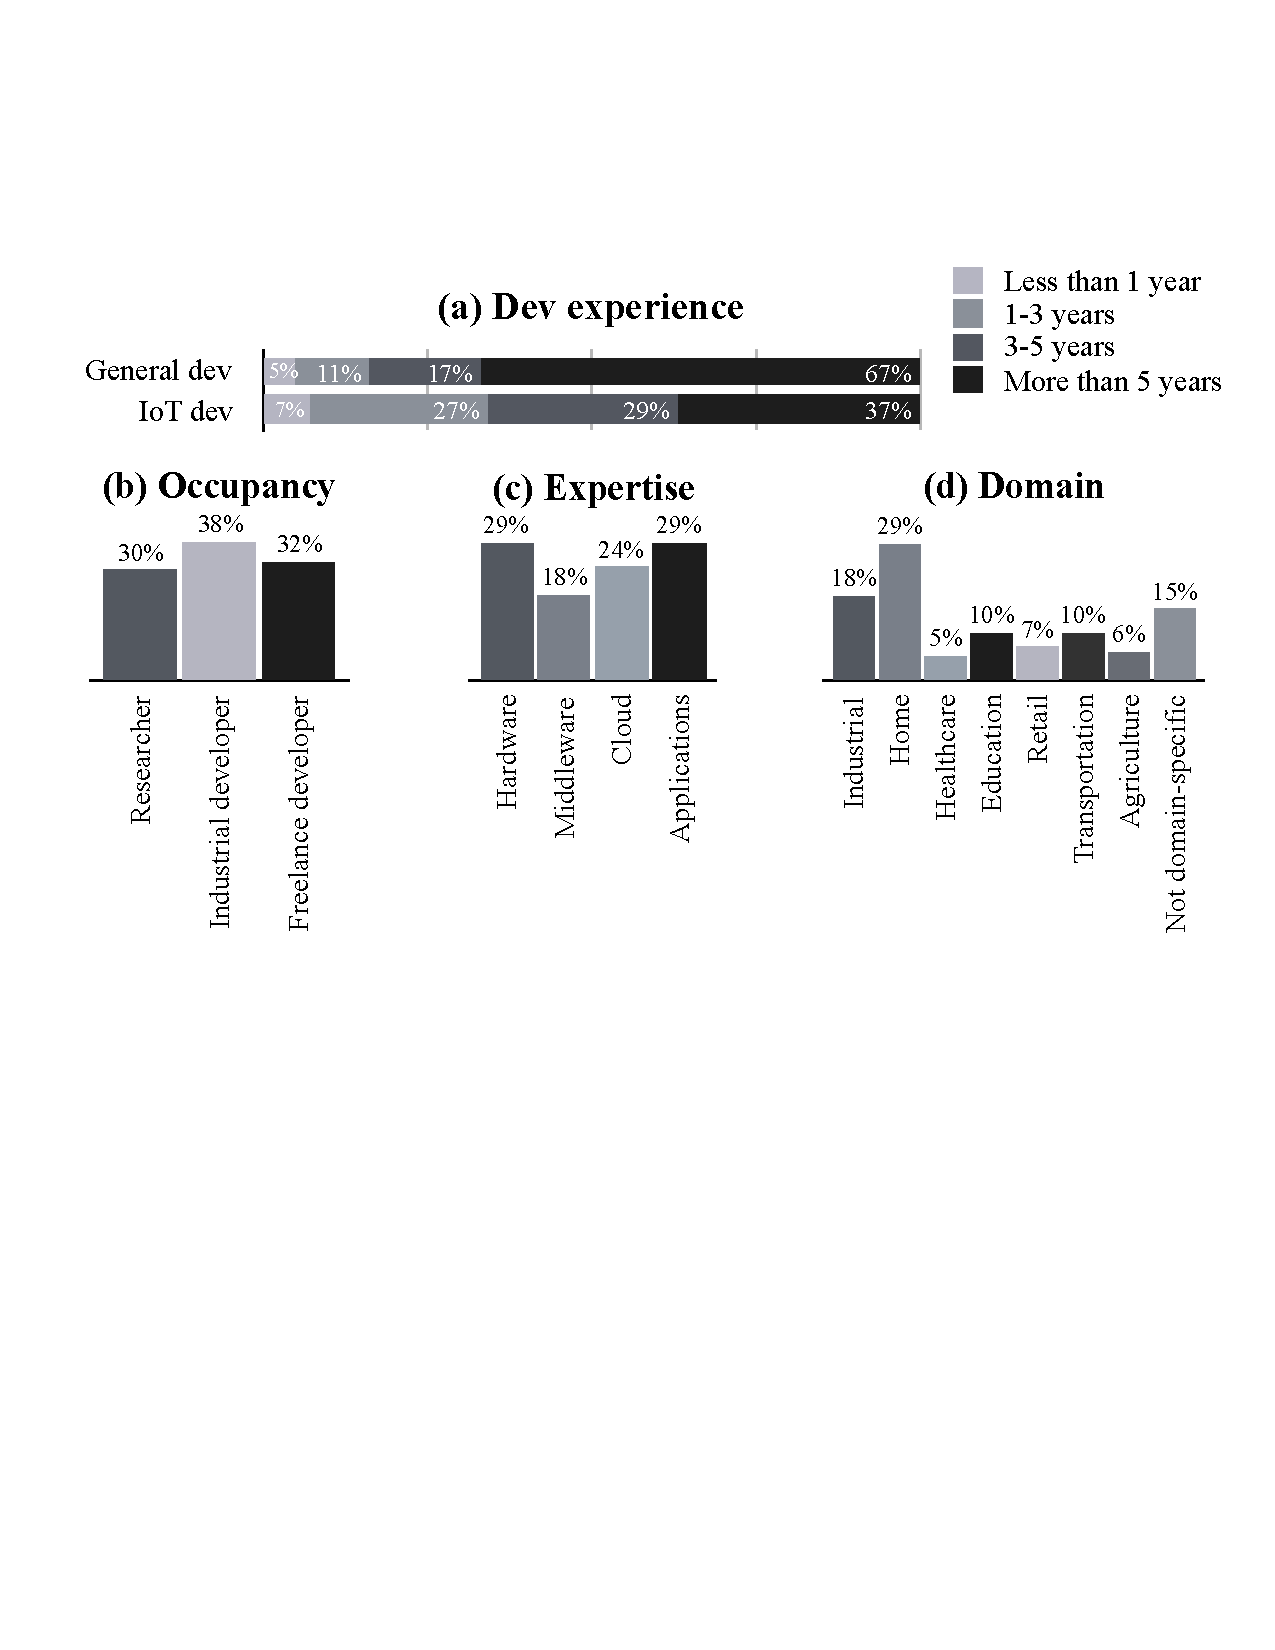
\includegraphics[width=\linewidth]{imgs/demog.pdf}
  \caption{Development backgrounds of the survey participants}
  \label{fig:demog}
\end{figure}

\textbf{Protocol}
The survey has three sections. In the first section, we collect participants' background in IoT, and in general development, which is depicted in~\autoref{fig:demog}. The second section concerns the challenges of developing IoT systems with questions aimed at correlating our findings with the participants' own experiences. 

The third section is about the frequency and severity of bug categories based on participants' previous experience in IoT development. At the end of each section, there are open-ended questions to allow them to share their comments about our results and mention new categories.

\textbf{Analysis}
Our survey was completed by 194 respondents, with a response rate of around 10\% for valid responses. 
 We received 95 comments through the open-ended questions sections. All of the survey respondents' comments are coded and analyzed following the same procedure discussed in \autoref{interviewAnalysis}.

\section{Findings: IoT Bug Categories (RQ1)}
In this section, we describe our findings regarding IoT bugs. 


\subsection{Taxonomy of Bugs}
We used all the tags collected by RCA of the bug reports in our dataset, to build a taxonomy of bugs in IoT systems. As our motivating example illustrates~\autoref{motivExample}, IoT bugs can be multi-faceted and manifest at different layers and locations. Therefore, we designed our bug taxonomy to accommodate all these bug characteristics. Considering various approaches suggested by Usma et. al.~\cite{usman2017taxonomies} for taxonomy construction, we followed the approach suggested by Kwasnik~\cite{kwasnik1999role} as IoT bugs are multi-faceted and relatively a new and unexplored concept. Following their approach, we first defined facets of our classification as all failures and locations of failures. Then, we analyzed all bug reports based on these facets and built a hierarchical taxonomy that accommodates all the dimensions.

After we built the initial version of the taxonomy, we used the data from the interviews and the survey to complement and enhance the taxonomy. We reviewed all previously tagged data and re-tagged them after each alteration of the taxonomy. \autoref{bugTax} depicts our IoT bug taxonomy. Next, we describe the major bug categories in our taxonomy. We will use specific bugs as examples for each category. All these bug examples are available in our dataset, which is available online~\cite{repPack}. 


\textbf{IoT Device}
This category of taxonomy covers bugs that are related to IoT device hardware and firmware.

\textit{Device hardware:}
Bugs in this subcategory are related to the physical aspects of IoT devices.  Examples include bugs related to wiring issues, device pin status issues, or issues with physical sensors and actuators of the device. For example, PEDALINOMINI/34 is related to the device not differentiating between single and double presses of a hardware button. 
 
 Other common bugs in this category are those that are linked to the device's limitations in memory, power consumption, or processing capacity. One such instance provided by P\textsubscript{1} as he described a scenario where a device on low battery generated incorrect data to the cloud. There are various similar cases in our collected bug reports where the low battery of the device or the removal of the power source of the device causes failures. Even in some cases, enabling power saving mode cause unexpected behaviours such as variable lag. For example, in DEVICE-OS/1567, the power saving mode causes some variable lag, which led IoT developers to disable the power saving mode as they had not accounted for such delays.
 
 Another group of device hardware issues is the problems regarding booting or rebooting the device. For example, heavy calculations and processing on the device (HOMIE-ESP8266/575, interviewee P\textsubscript{8}) cause a device boot loop issue. Also, there are cases where the IoT device runs out of memory (ZWAVE2MQTT/141, interviewee P\textsubscript{7}) which are other types of bugs related to this category. Another example of known hardware issues of IoT devices is the known timing issues of Raspberry Pi devices~\cite{piClockissues},  which is also mentioned by an interviewee (P\textsubscript{8}).

\textit{Device firmware:} 
Firmware bugs consist of three subcategories. The first pertains to device firmware unexpected exception and hang issues. The second sub-category includes issues related to the configuration of the IoT device, which can be specified as an external instruction sent to the device for a specific purpose. This type of bug usually happens in the early stages of introducing an IoT device to the IoT network. Each device has to be configured properly in a way to be compatible with other hardware or software components and also be able to communicate with others on the network. Issues associated with configuring the device with WiFi credentials or with configuring the device with the correct firmware version are some common examples here. The third and most common sub-category is the firmware upgrade issue. There are various cases where poor practices for handling over-the-air (OTA) updates of the device firmware, stale updates, or updating the device firmware with the wrong binary have caused failures of the IoT system.
In some cases, the stale update issues are related to device configuration issues as in WTHERMOSTATBECA/54, where the device needs to be re-configured with WiFi credentials after each firmware update, otherwise, future firmware updates would be stale. 

\textbf{Compatibility}
When a bug occurs only on a specific type of device, communication protocol, or third-party component, it falls under the compatibility category. For instance, a common device incompatibility issue happens when certain devices represent their telemetry data in different formats, leading to the other components not being able to process their data. Other common bugs are linked to compatibility issues of certain combinations of sensors and development boards, e.g., incompatibility of the DHT temperature sensor with the ESP32 microcontroller in MONGOOSE-OS/277. Issues with the interoperability of different protocols is another case. One example is MAINFLUX/1079, which is related to the interoperability between the HTTP and MQTT protocols. A common bad practice in IoT development related to these issues is developing protocol-specific or device-specific code. For instance, in DEVICE-OS/1938, the IoT platform relies on event components to report what protocols each event is intended for, in order to be able to run different functions for each protocol individually. However, sometimes developers have no other choice but to follow this error-prone approach, just to bypass the limitations of third-party devices. For instance, (P\textsubscript{2}) mentioned a case where the incompatibility of the Raspberry Pi and some types of sensors had forced their developers to implement custom logic for the communication of these devices. Developers had to switch between Raspberry Pi's default implementation and their own custom implementation based on the sensor type, leading to many issues.

\afterpage{%
\begin{figure*}%[ht]
  \centering
   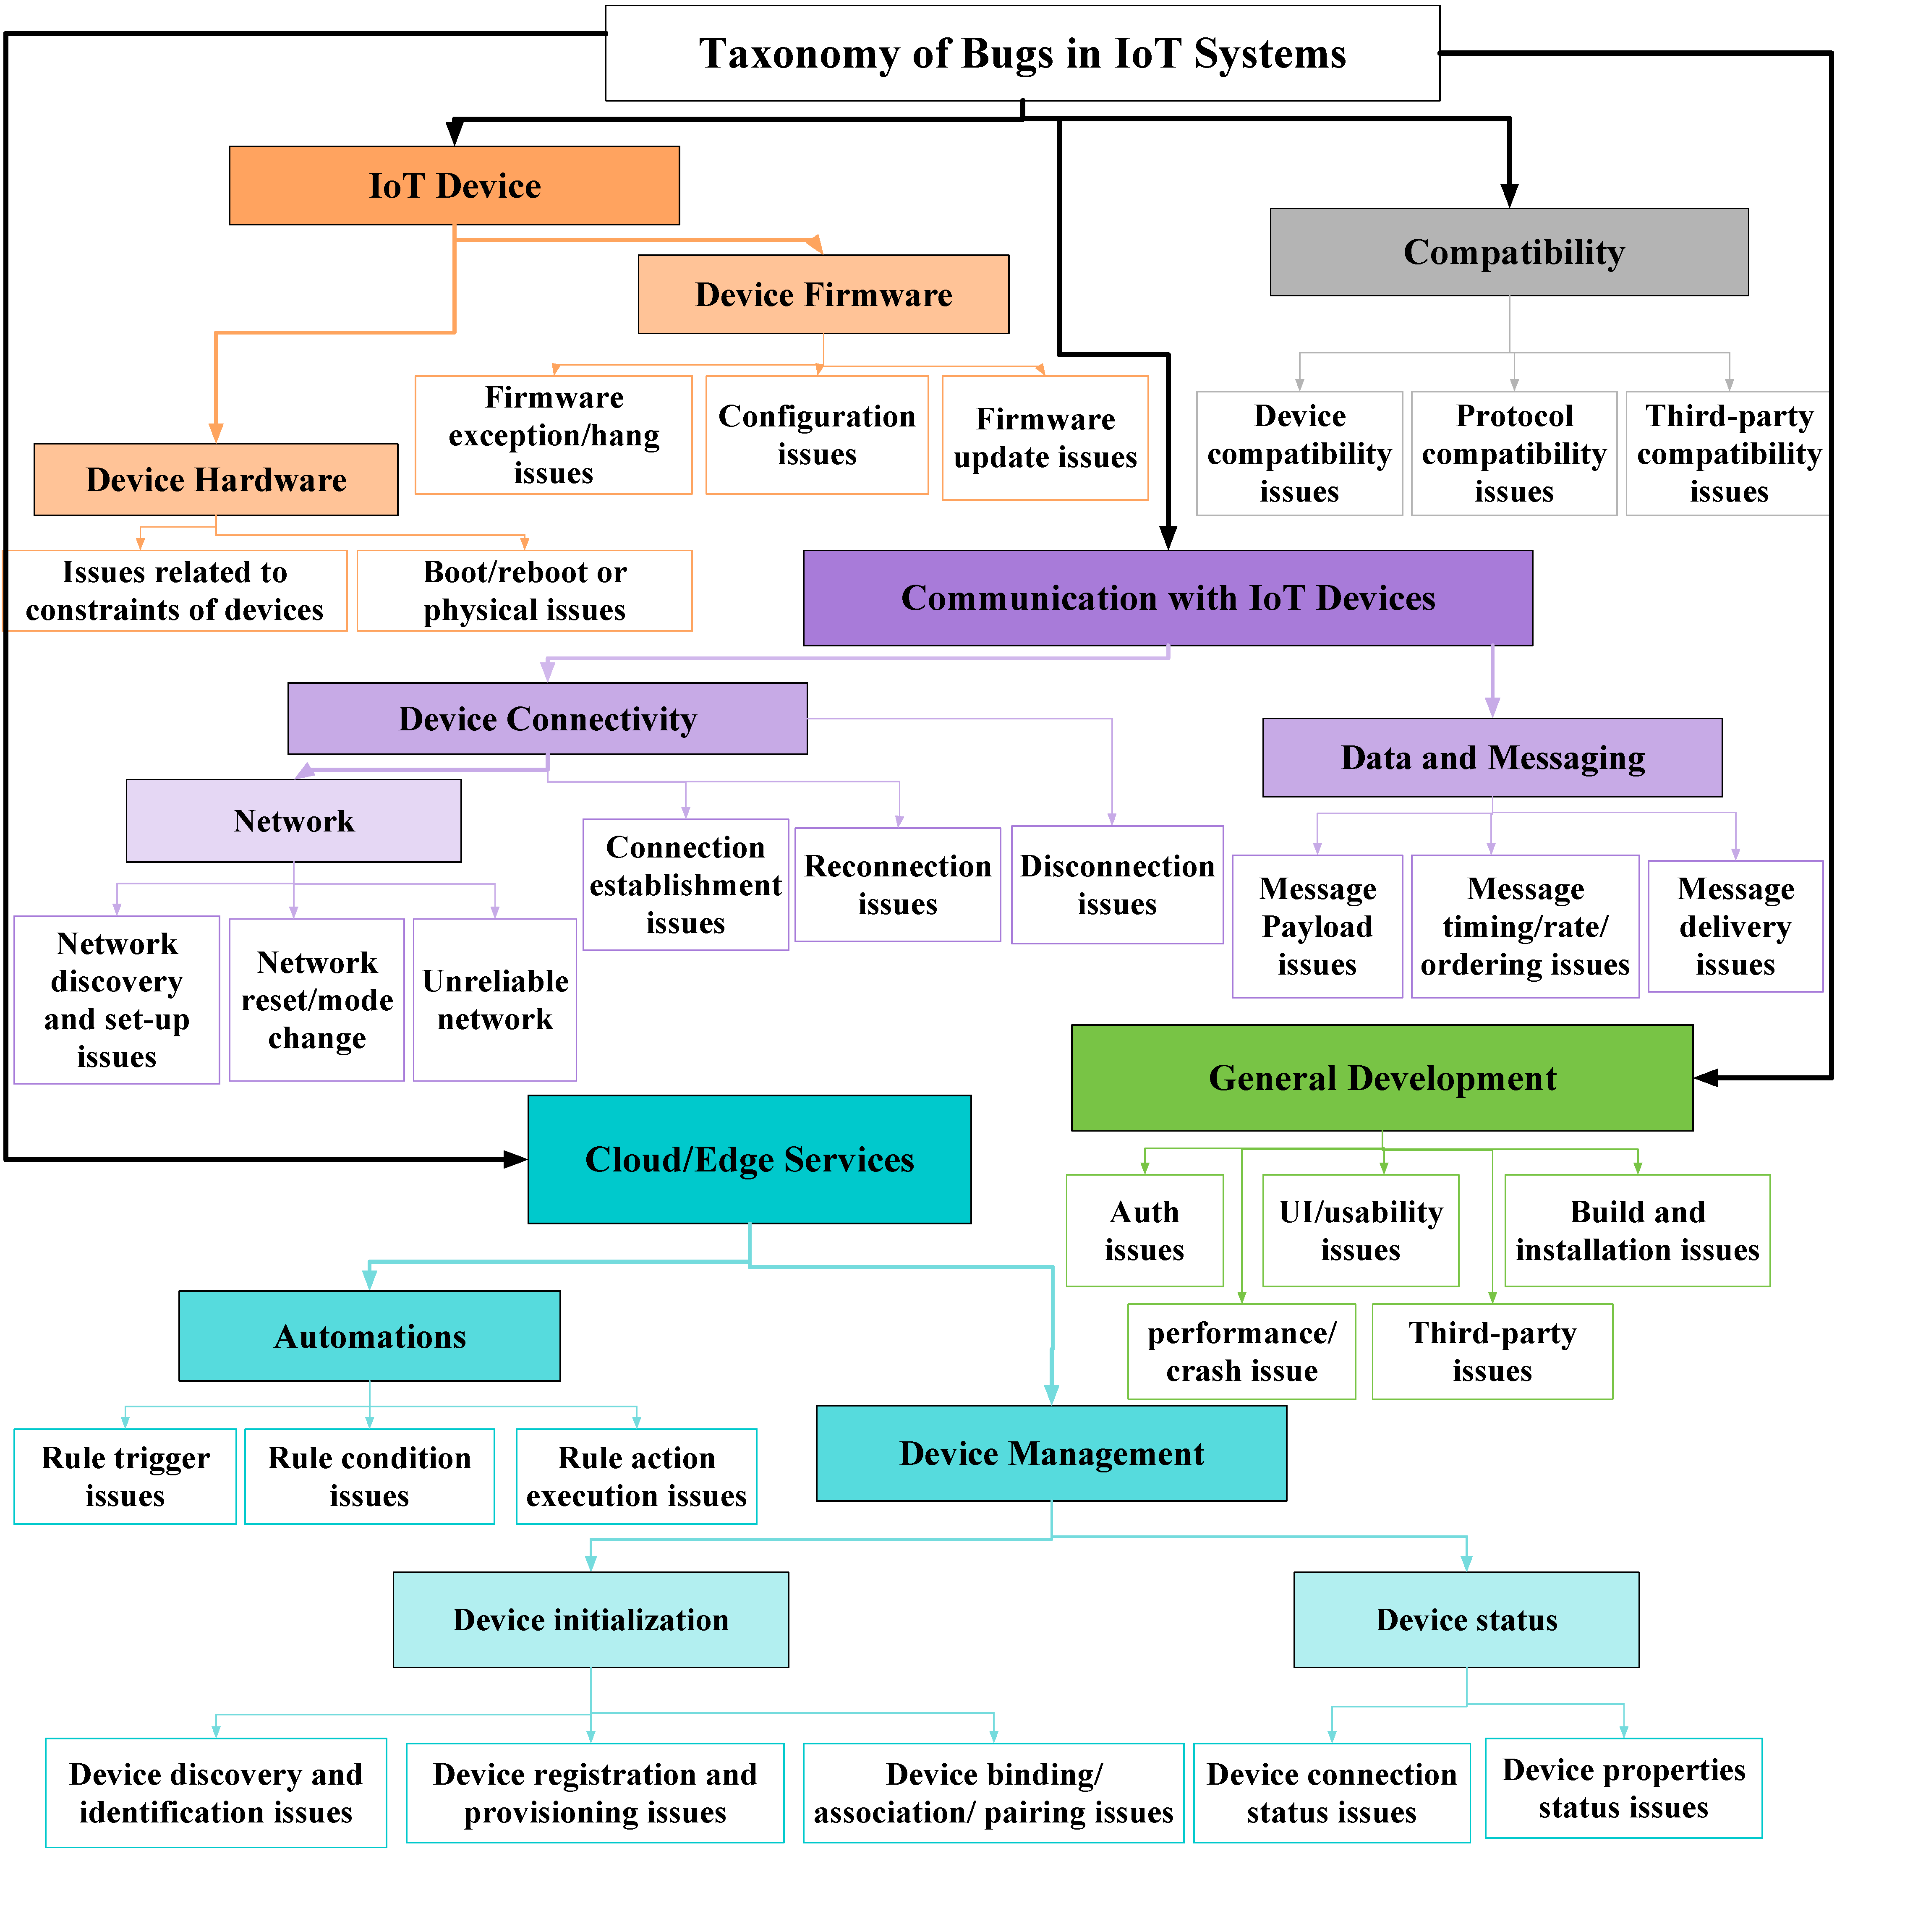
\includegraphics[width=\linewidth]{imgs/tax.pdf}
  \caption{Taxonomy of IoT bugs.} 
  \label{bugTax}
\end{figure*}
\clearpage
}

\textbf{Communication with IoT devices}
Bugs that are related to the communication of IoT devices with each other or with other entities fall under this category. Generally, there are two types of bugs in this category:

\textit{Device Connectivity:} 
Some of the connectivity issues are related to the network that the device relies on for connecting to the internet. One example is when the device cannot discover a valid and available network such as a local access point and therefore loses access to the internet. As it is also mentioned by P\textsubscript{9} \enquote{When the device location is changed to another room or another building, the device has to be reconfigured for the new access point.}

\begin{lstlisting} [language=Java, caption={An example of testing a bug fix after WiFi reconnection in DEVICE-OS/1639}, label={lst:wifiReset}] 
// Initial Wifi Connection
  WiFi.connect();
  // asserting socket creation are done correctly
 const sock_handle_t sock = socket_create();
  if (!socket_handle_valid(sock))   Log.error("socket_create() failed");
 // Asserting that socket connection works without error
 const auto r = socket_connect();
  if (r != 0)  Log.error("socket_connect() failed");
<@\textbf{// WiFi Reconnection and asserting the socket closure operation}@>
 WiFi.off();
 WiFi.connect();
const auto r2 = socket_close(sock);
if (r2 != 0)  Log.error("socket_close() failed");
\end{lstlisting}

 
In addition to the network discovery, not handling a network reset, or unstable and unreliable networks are other common issues that can lead to failures. However, Sometimes IoT devices fail to establish a valid connection to the gateway or remote cloud servers despite a valid network status. Failure in reconnecting, connection refreshing, and ensuring such connectivity failures do not cause propagated failures in other components are other pitfalls that IoT developers often deal with. Additionally, unexpected disconnection or connection closure issues are other manifestations of bugs in this category.

Listing~\autoref{lst:wifiReset} shows a real-world example of the additional tests IoT developers write to check if a fix for a bug caused by WiFi reconnection is a good enough fix. As this example shows, IoT developers have to write code that is able to handle unexpected reconnections and disconnections in order to avoid connectivity bugs.

Additionally, two interviewees (P\textsubscript{6} and P\textsubscript{9}) believe that connectivity bugs are the most serious and challenging bugs. As P\textsubscript{9} states \enquote{the weakest part of our IoT platform is to communicate with IoT devices.}

\textit{Data and Messaging:}
This category includes bugs that are related to data and message sending in the IoT system. Typically, messages are either commands that are sent to IoT devices via the cloud, or they are telemetry data that are received from IoT devices in the edge, cloud, or applications. Some bugs cause failures in delivering these messages from the sender to the receiver. Some other messaging bugs are related to the timing of messages. For instance, various reported bugs are related to the rate and order of the messages. Additionally, some bugs are linked to the payload that is being delivered through the messages. 

In some cases, payload size or format are the causes of failures. There are also cases where there are violations of payload integrity by messages being truncated or overwritten. For instance, in HOMIE-ESP8266/309, the IP address is truncated by one character in the MQTT response message.


\textbf{Cloud/Edge Services}
This category includes bugs that are related to the services delivered by the remote cloud servers or gateway devices in the edge layer. 

\textit{Device Management:}
To monitor and control each IoT device remotely, devices should be connected to a cloud server or a hub device, and report their status while listening to user commands. Device management (DM) issues include problems that cause failures in this process. 
The first class of DM issues happens in the stage of initializing the IoT device in the cloud or edge systems. One type of device initialization (DI) issue is when the IoT device is not properly or uniquely identified by the cloud or edge components and therefore causes further failures in the subject IoT system. Besides, if the IoT device fails to provide a recognizable identity and valid permissions to the cloud or edge, it would not be allowed to use remote services. Some examples of device registration and provisioning bugs are duplicate device certificates, issues with auto-provisioned devices, or failure in retrieving data from the provisioning service. Another class of DI bugs is problems with binding, association, and pairing of IoT devices. There are several cases where bugs are introduced to the IoT system just because devices are grouped together (such as devices in one room), due to not properly handling the association of a sensor device with a physical object. There is an example mentioned by one of our interviewees (P\textsubscript{5}) where two switches were associated with one lamp and only one switch was working due to issues with addressing multi-instance devices with labels.

The second class of DM issues is related to problems with monitoring the status of IoT devices. One type of device status is the connectivity status, to check whether the device is online, which is also known as the heartbeat check. Some examples of bugs in this type are wrong device heartbeat rate, showing a lost connection as live and vice-versa, or not notifying other components when the device goes offline. Failure in retrieving the device status such as color and brightness for a light bulb, showing the status incorrectly, or failure in updating the device status are some examples of these types of issues.

\textit{Automation:}
This bug category is related to automation services that IoT cloud or edge platforms provide and it is classified into the trigger, condition, and execution issues. Rule trigger defines a condition under which a rule is initiated. Trigger failures usually cause a rule not to become triggered when it should be (SMARTHOME/5578) or vice-versa (HOME-ASSISTANT-CONFIG/2). Rule condition is the statement that should be checked when the rule is triggered. Examples of the rule condition issues are problems in retrieving the device state to check the rule condition since the condition usually relies on device latest status (TESLA-API/43). Issues in the execution of the rule action are the last and the most prominent automation issues. Some examples of these issues are crash after rule action execution, issues in handling asynchronous behavior and threads in rules, and having problems with the output of the rule being unpredictable or nondeterministic.

\textbf{General Development}
This category captures common development bugs. Some common issues are problems with installing, compiling, or building a project as well as unexpected crashes or performance issues in the IoT project. The general development category also includes bugs in the authentication or authorization process. One of the IoT-specific authorization issues are problems with generating, signing, or maintaining the certificates that devices have to present for using cloud or edge services (AZURE-IOT-SDK-C/657). Other sub-categories of general development bugs are UI-related, usability, or external issues.

\subsection{Root causes of Bugs}

\afterpage{%
 \begin{figure*}
  \centering
   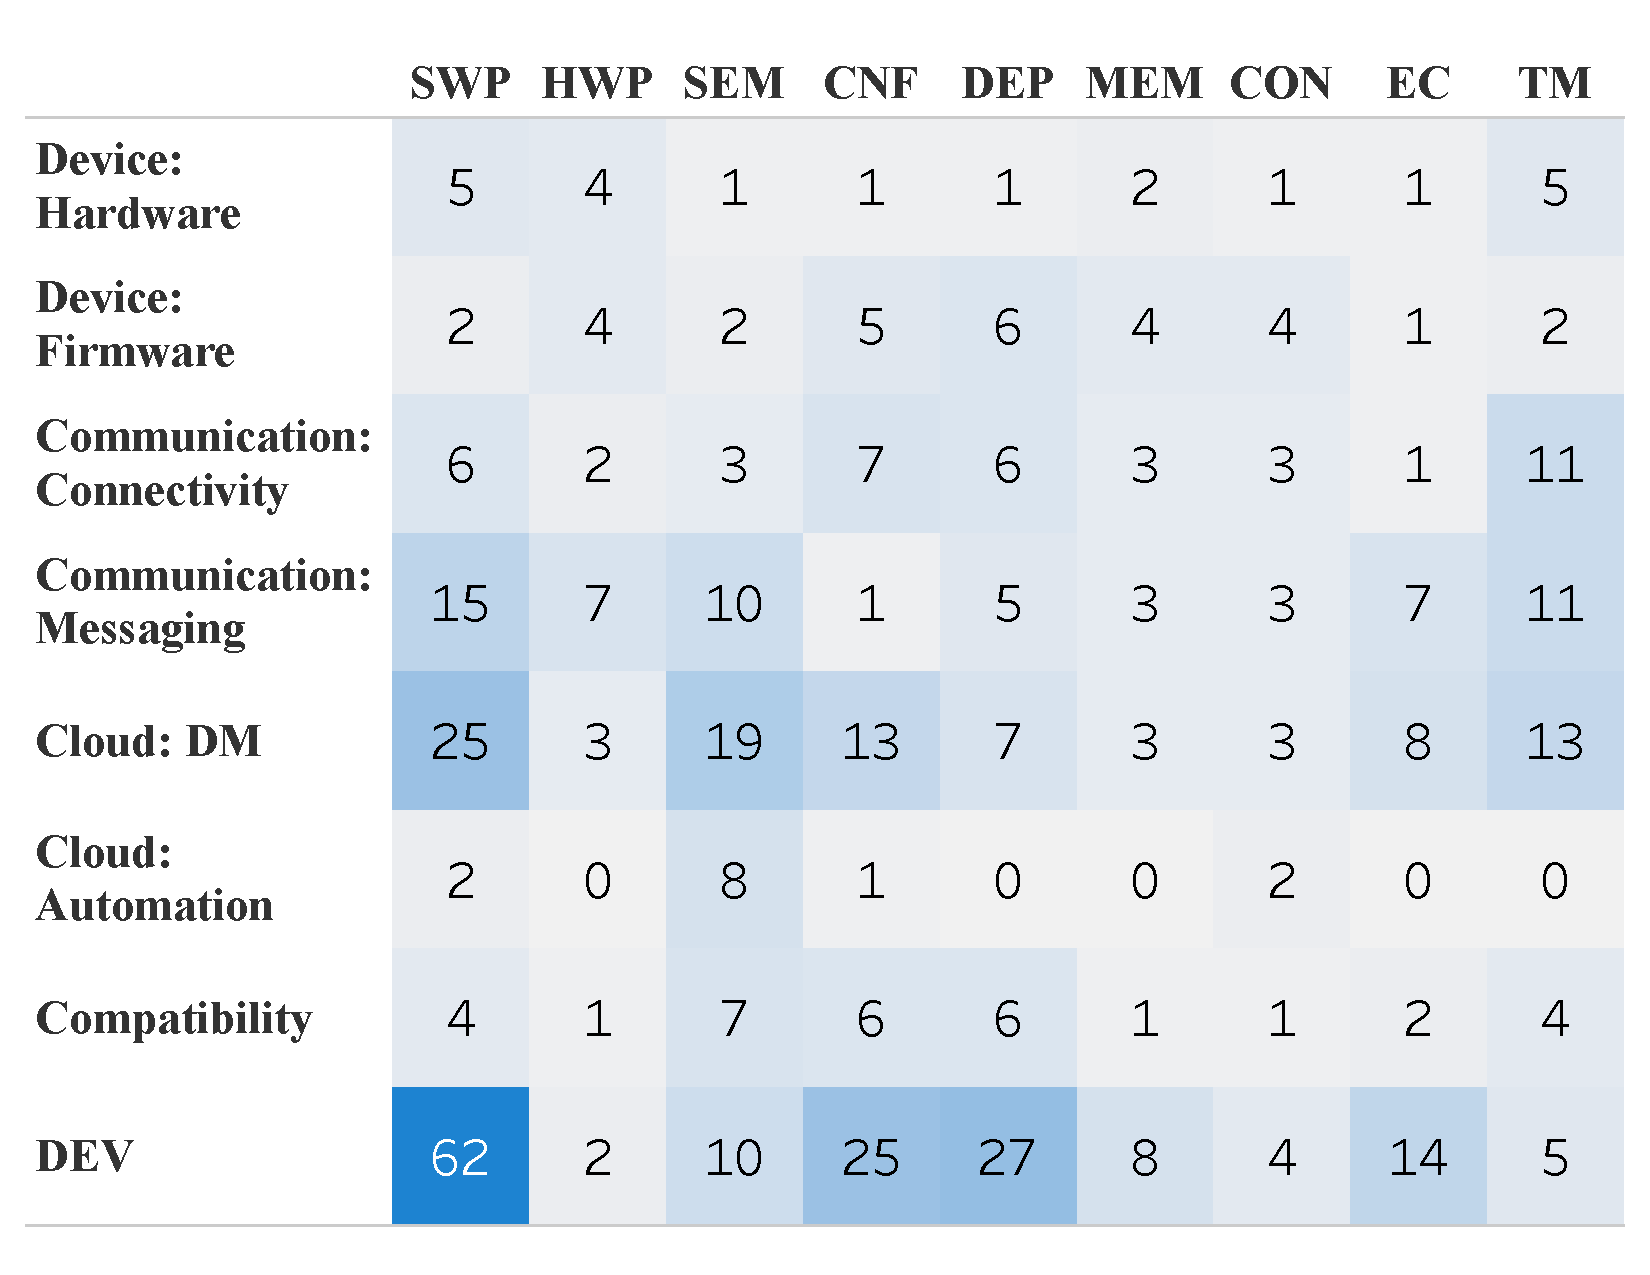
\includegraphics[width=\linewidth]{imgs/rcvis.pdf}
  \caption{Distribution of bug categories (vertical) and root causes (horizontal)}
  \label{fig:bugRC2d}
\end{figure*}
\clearpage
}

Figure \ref{fig:bugRC2d} shows the distribution of bug categories and root causes. In this section we will describe each category of root causes. 

\textbf{General software programming faults (SWP)}: These faults are the most dominant root causes of the bugs. These faults are often syntactical mistakes by IoT developers. Examples of such faults would be accessing null pointers or empty memory locations, typos, missing/wrong conditions/loops, or missing/wrong values in code, infinite loop, and wrong data type. Also, we consider all UI-related faults to be in this category, like faults in the front-end code of a web application or an Android or iOS application. The top three issues caused by these faults are messaging issues, device management issues, and general development issues.


\textbf{Semantic programming faults (SEM)}: These faults are the second most dominant root causes of IoT bugs. After general development issues, top issues caused by SEM faults are device management issues, automation issues, and compatibility issues. Some semantic mistakes that IoT developers make are wrong control flow, faulty logic of functionalities, or erroneous return values. 

Among SEM related faults, wrong return values are one of the most challenging one to deal with for developers. One example of faulty return values is the mistake in AZURE-IOT-SDK-C/481, when the developer wants to get a device with a certain ID. If the device ID does not exist, the expected behaviour is to create a new device with that ID and return the newly created device. However, if a device with a certain ID does not exist, the IoT platform mistakenly returns an error code which is a fault in the return value. Also figure\~autoref{fig:sem} is about bug report SYNSE-SERVER/91, which occurred in an IoT plugin SDK. Developers are struggling to identify the expected behaviour of the IoT system when facing empty messages from devices. Their observations suggest that empty messages from devices might sometimes mean that the device is misconfigured. As a result, developers have to check whether the empty message is from a previously configured device or not.

 \begin{figure}[ht]
  \centering
   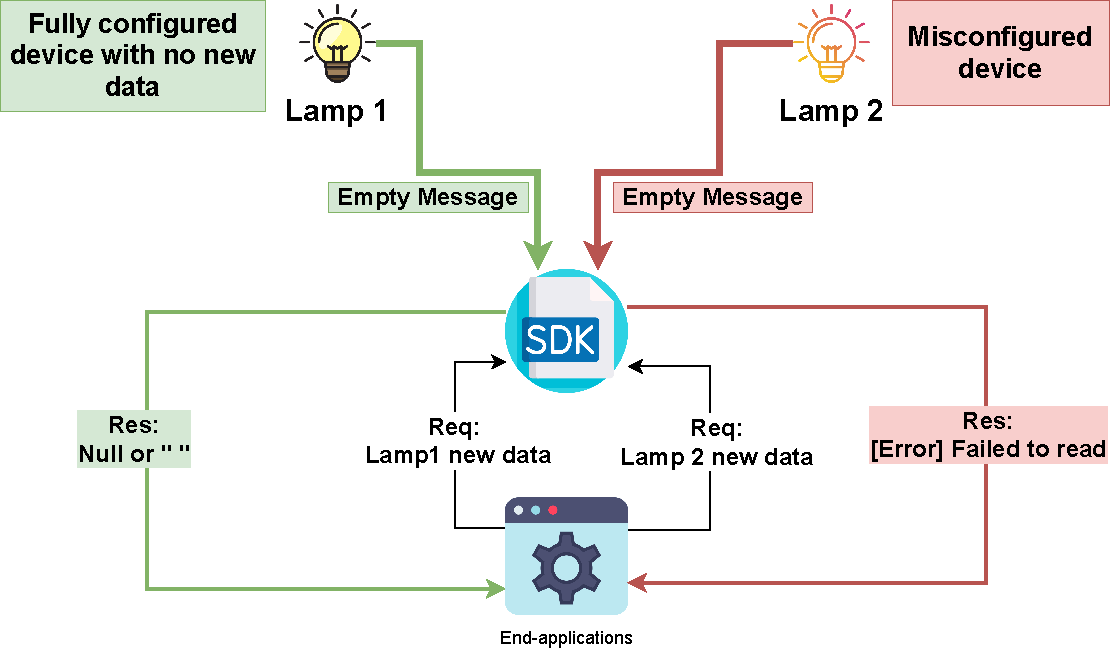
\includegraphics[width=\linewidth]{imgs/sem.pdf}
  \caption{The IoT SDK should not treat the empty messages from device 1 and 2 in the same manner. To avoid making a SEM fault by returning a wrong value to end-applications, the SDK developers have to check whether the requested IoT device has been previously configured or not. This figure shows the correct expected behaviour.}
  \label{fig:sem}
\end{figure}

Some SEM faults are related to the automation logic of the IoT system, such as logical faults in automation apps, which are also discussed in recent studies~\cite{ISSTA2020Interactions}.  An example of such mistakes is obvious in ENTITY-CONTROLLER/103, where developers have conflicting opinions on the expected behaviour of IoT devices when an overriding command is sent to devices. This issue gets more serious when the expected behaviour designed by developers as the correct behaviour, does not support certain user scenarios, which is the case in this bug example.

\textbf{Dependency faults (DEP)}: The next frequent root cause is DEP faults, where developers use wrong versions of the software or firmware libraries, tools, devices, or protocols. Dependency faults are the main causes of compatibility issues, device firmware issues, and general development issues. It's important to note that dependency faults are different from compatibility bugs in nature since the latter is mostly an observed failure that can have different causes (as we can see in \ref{fig:bugRC2d}), where the first one is a fault by developers in choosing the right version. Developers have to follow the dependency constraints among hardware devices and software libraries to avoid these faults in their code.

\textbf{Timing faults (TM)}: One of the most important root causes often leading to hardware, connectivity, and messaging issues are TM faults. Improper handling of time-outs or rate of operations, wrong time-out values for connection closures, or not handling asynchronous behaviors are among timing-related root causes. In some cases, the connection is monitored to be closed when the device is idle. Furthermore, finding the ideal time-out value for properly closing the connection to avoid possible failures has shown to be a faulty task for IoT developers.

One example of TM faults occurs in DEVICEHIVE-JAVA-SERVER/145 when users want to get a specific command of a certain device and instantly receive an empty array as the response when the device is still busy executing the same command from before. The expected behaviour is to wait until the device acknowledge the complete command execution within the defined time-out. Figure~\autoref{fig:tm} shows part of the bug fix for this issue, that enforces the device to first wait for the command to be processed.

 \begin{figure}[ht]
  \centering
   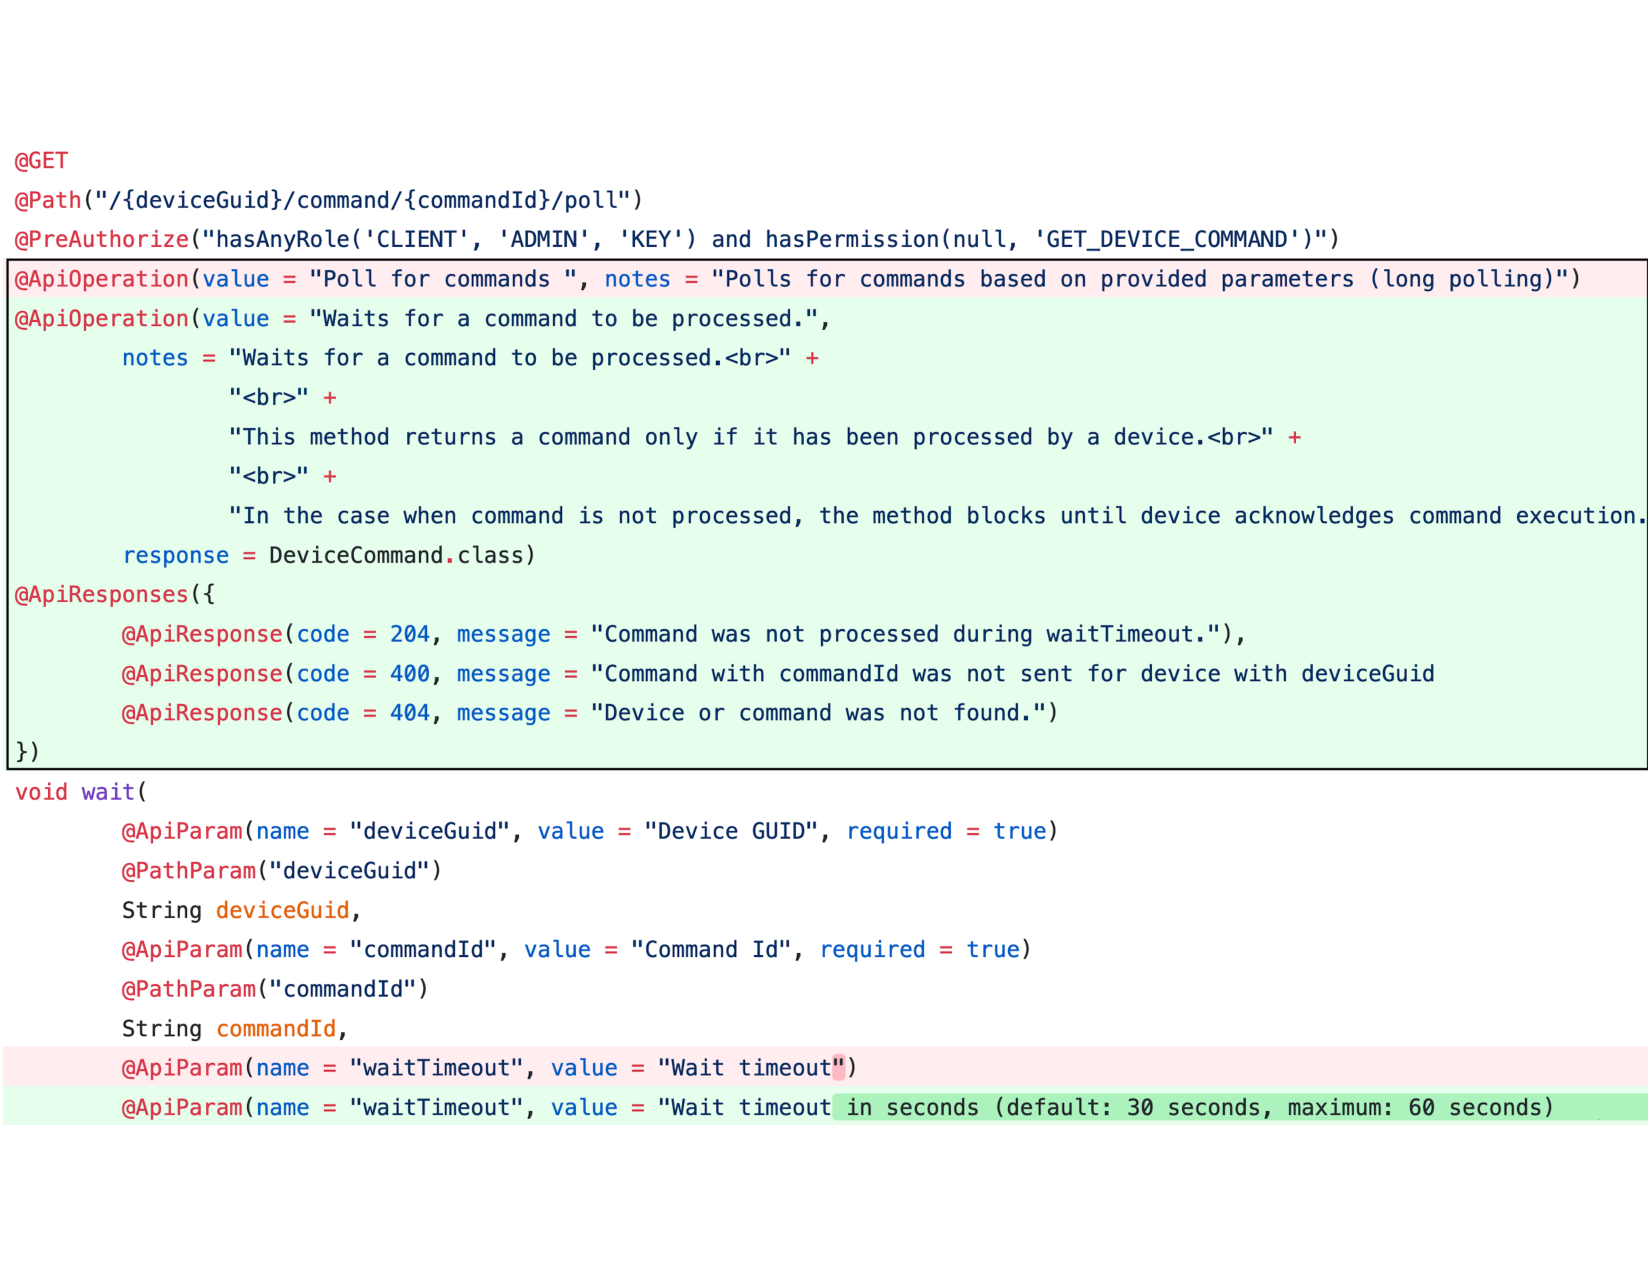
\includegraphics[width=\linewidth]{imgs/TM}
  \caption{A timing fault while polling device commands occurred in DEVICEHIVE-JAVA-SERVER/145}
  \label{fig:tm}
\end{figure}


\textbf{Hardware programming faults (HWP)}: Some faults that are more specific to hardware programming such as interrupt handling, are assigned to the category of HWP faults. Examples include wrong pin/port mapping, improper socket operation, wrong bit assignment, and incorrect interrupt handling. Other faults in hardware code resemble those in software code, like referencing a null pointer or wrong return type.

\textbf{Faults in handling exceptional cases (EC)}: These faults are another root cause for IoT bugs that include mistakes in handling corner cases (large or out of range data), not handling errors properly, or not handling changes of the requirements or changes in third-party components. Figure~\autoref{fig:rc8} shows a EC fault in which the IoT developers did not count for large messages.
 
 \begin{figure}%[h]
  \centering
   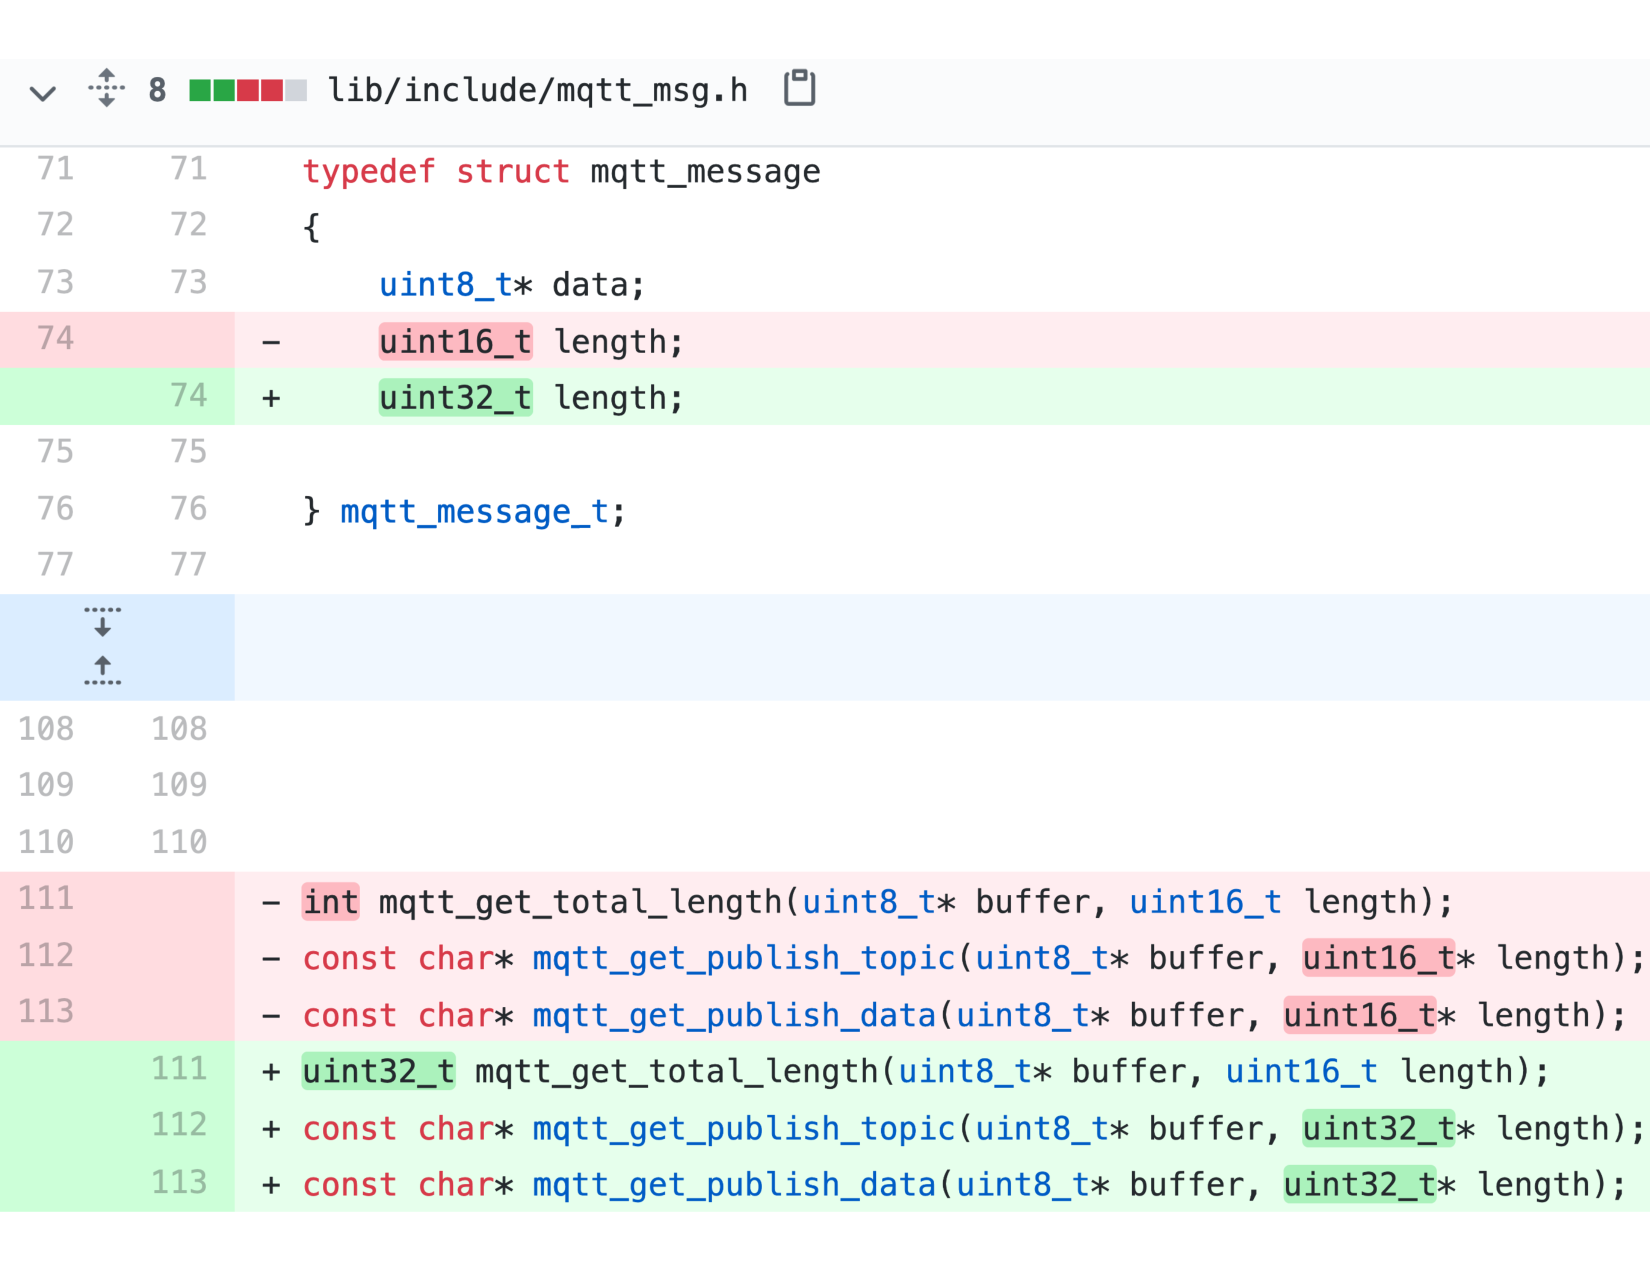
\includegraphics[width=\linewidth]{imgs/rc8}
  \caption{An EC fault (from ESP-MQTT/34) that allocates 16 bit instead of 32 bit for each MQTT message, which cause the system to break with large MQTT messages.}
  \label{fig:rc8}
\end{figure}
 
\textbf{Memory faults (MEM)}: Faults related to incorrectly handling memory objects fall into this category. There are some previous studies focused specifically on memory-related bugs \cite{memBugs}. Also some other studies have categorized these bugs as a defect in software systems \cite{openSourceBugs}. Memory bugs often happen as the result of race conditions on memory locations. A race condition is a situation in which the result of an operation depends on the interleaving of certain individual operations. Such situations can lead to different types of bugs like buffer overflow, stack smashing, memory leak, uninitialized read, and double free bugs, as it is also classified in bugBench \cite{bugBench}.

\textbf{Concurrency faults (CON)}: A concurrency fault exists if running two threads at the same time is not handled properly. These faults usually do not show up if the two programs run sequentially. Thus, these bugs happen only in multi-threading or multi-processes environments and only when the operations are ill-synchronized. In the context of IoT, the communication of things and the cloud can be asynchronous, which means data can be transmitted intermittently rather than in a steady stream, because there are various parties (user, sensor, actuator) that can send data whenever they like. Based on the classification in bugBench, there are three types of concurrency bugs. Data race bugs happen when at least two threads access a shared variable at the same time. At least one thread tries to modify the variable. Atomicity-related bugs happen when one thread is unexpectedly interrupted by another thread. Deadlock is a situation when two or more threads wait for a resource and can never proceed anymore. 


\textbf{Configuration faults (CNF)}: Hardware devices and development tools need some particular configuration, and wrong provisioning of the proper configurations are considered CNF faults.


\subsection{Correlations among bug categories}
During our analysis, we observed some frequent patterns of certain bug categories appearing together more often. To study the correlations between bug categories, we used Lift~\cite{kamber2001data}, a statistical metric introduced by Han and Kamber that computes the probability of two categories appearing together. For each pair of bug category, a lift value of more than 1 shows a positive correlation, and a lift value below 1 reveals a negative correlation. 

Table \ref{tab:correlations} shows the lift values of correlated bug category pairs. The top correlated bug categories are [hardware, firmware], [hardware, connectivity], and [firmware, connectivity]. This correlation analysis, besides helping IoT developers in debugging, gives insight into how intertwined IoT bugs can be in practice.


 \begin{figure}%[h]
  \centering
   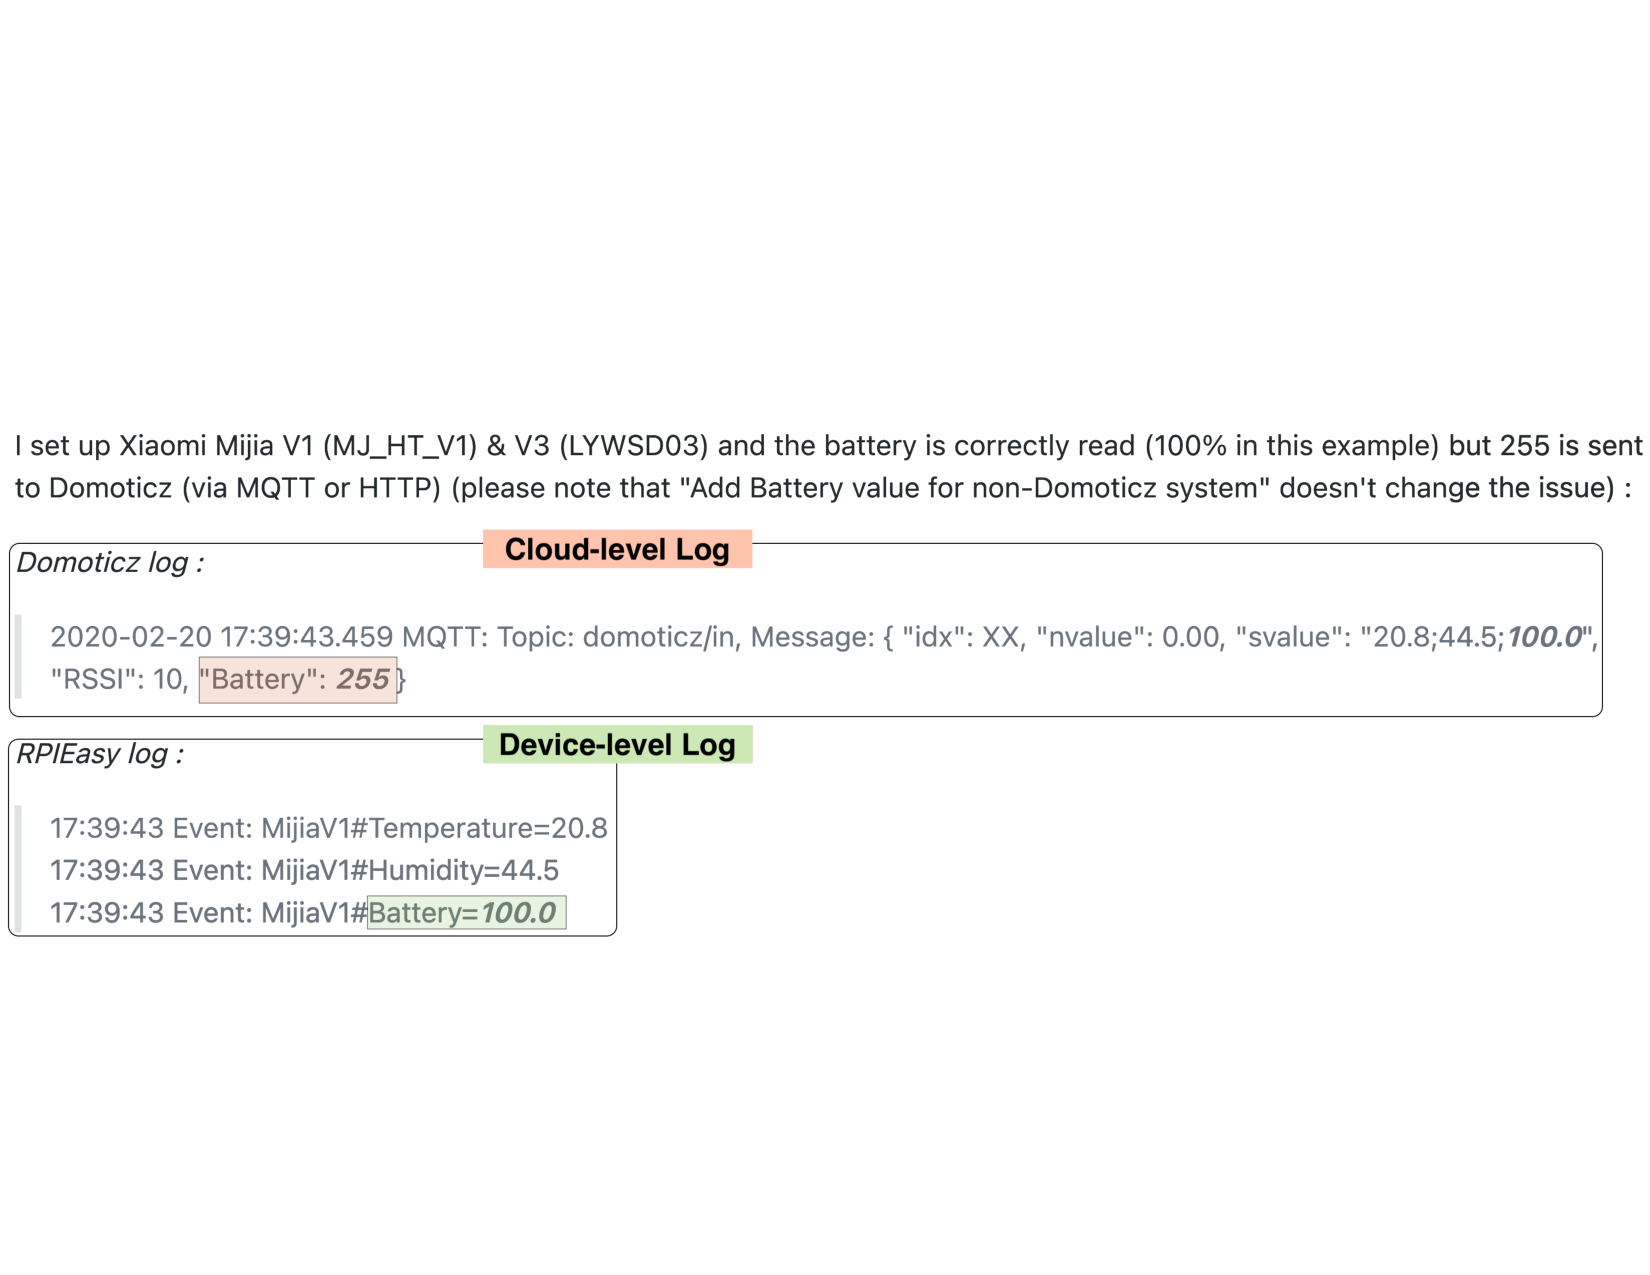
\includegraphics[width=\linewidth]{imgs/corEx}
  \caption{An example of how a fault in the device layer has propagated to a failure in the cloud layer}
  \label{fig:corEx}
\end{figure}


As the Figure~\autoref{fig:corEx} shows the GitHub discussions for RPIEASY/128, an IoT developer observed a clear conflict between the device status logged from the device layer and the cloud layer. Further investigation revealed that a fault in the device driver code has caused the wrong device battery status to be sent to the IoT cloud.

 \begin{table}[htbp]
\caption{Bug Categories with Positive Correlation}
\begin{center}
\resizebox{\linewidth}{!}{%
\begin{tabular}{l l | r}
\hline
\textbf{Bug Category}& \textbf{Bug Category }& \textbf{Lift Value}  \\
\hline
Device: Hardware& Device: Firmware& 3.86   \\
Device: Hardware &Communication: Connectivity & 2.57   \\
Device: Firmware &  Communication: Connectivity & 2.25   \\
Compatibility &  Cloud: Device Management & 1.84   \\
Compatibility &  Communication: Messaging & 1.44   \\
Communication: Messaging & Device: Firmware  & 1.42   \\
Cloud: Device Management & Automation  & 1.38   \\
Cloud: Device Management & Device: Hardware  & 1.28   \\
Communication: Connectivity&Communication: Messaging & 1.22   \\
Communication: Connectivity& Compatibility & 1.14   \\

\hline
\end{tabular} }
\label{tab:correlations}
\end{center}
\end{table}


\subsection{Frequency and severity of bugs}

The most frequent categories of bugs are general development issues (48\%), device management issues (29\%), and messaging issues (19\%). 

We asked our survey participants whether and how frequently they face each bug (sub)category and what are their perceived severity based on the impact on the IoT system and fixing-time. Table \ref{tab2} shows the results.  All the bug categories in our taxonomy have been faced by at least 82\% of IoT developers, which shows the bug categories are representative of the real-world bugs in IoT systems. Connectivity issues are the most frequent and severe bug category with more than 97\% of IoT developers have faced it at least once. more than half of developers face it frequently, and 62\% of IoT developers find it severe. After this category, messaging, automation, and device management issues are among the most approved bug categories with all of them approved by more than 90\% of IoT developers. 

In terms of frequency, hardware, and messaging issues are among the most frequent bug categories after connectivity issues. 

Device-related issues are the least experienced bug categories, but they are the most severe bugs after connectivity issues. According to the survey respondents, automation issues are the least severe bugs, however, more than 91\% of IoT developers have faced them at least once. The compatibility issues are the least frequent bugs according to IoT developers' experiences.

Regarding sub-categories, device initialization issues are the most frequent and severe device management bugs since about 95\% of IoT developers having dealt with them, and more than half of developers find it severe. 

Also concerning the device status issues, bugs related to the status of connection have shown more frequency while bugs related to the status of device properties are more severe based on survey respondents. Among device-related issues, bugs that are related to the constraints of IoT devices have the most frequency. The device firmware exception issues are the most severe device-related bugs. Concerning general development issues, installation issues are the most frequent and severe bugs. 

Bugs related to authentication and installation are the least experienced general development bugs. Nevertheless, more than 81\% of IoT developers have the experience of dealing with them and nearly 30\% of survey respondents find this bug severe.


 \begin{table}%[htbp]
\caption{Survey Results: Bug Taxonomy}
\resizebox{\linewidth}{!}{%
\begin{tabular}{ l | r | r r r | r }
\hline
\multicolumn{1}{l|}{\textbf{Bug Category}} &\multicolumn{1}{l|}{\textbf{Have faced}}& \multicolumn{3}{c|}{\textbf{Frequency}}& \multicolumn{1}{c}{\textbf{Is Severe}} \\
& &Frequently&Sometimes& Rarely&  \\
\hline
Device: Hardware&82.50\% &30.30\% &39.06\% &30.64\% &43.61\%  \\
Device: Firmware&85.75\% & 24.20\%& 44.48\%& 31.32\%& 42.78\% \\
Communication: Connectivity& 97.22\% &50.29\% &38.29\% &11.42\% &62.78\% \\
Communication: Messaging&92.22\% &33.74\% &36.14\% &30.12\% &40.56\% \\
Cloud: Device Management& 90.93\% &25.06\% &46.43\% & 28.51\%&40.75\% \\
Cloud: Automation& 91.67\%& 20.00\% &44.24\% &35.76\% &32.22\% \\
Compatibility& 86.11\% &23.88\% &40.00\% &36.12\% &36.11\% \\
Dev&87.89\% &24.53\% & 39.44\%&36.03\% &38.89\% \\
\hline
\end{tabular} }
\label{tab2}
\end{table}

\textbf{Taxonomy augmentation}
Regarding IoT bugs, we collected 79 tags from interviews and 18 tags from the survey comments. Device binding issues, performance issues, and third-party compatibility issues were not discovered before the interviews and were added by interviewers' experience. The survey comments did not reveal any new information to be added to the taxonomy. However, the extracted tags, from both the interviews and survey, helped us to characterize each bug category by providing contextual data.


\subsection{Threats to Validity}
\textbf{Internal validity}
One internal threat to the validity of our study, similar to most qualitative studies, is researchers' bias in coding qualitative data. We mitigated this risk by having all authors of the paper involved in the tagging process and discuss any discrepancies in tags for all pieces of qualitative data from various sources (bug reports, interview transcripts, survey comments). For interviews specifically, we eliminated any personal preference on our results by triangulation; each piece of meaningful data from interview transcripts was tagged by one researcher who conducted the interview and one who was not present in the interview session.

\textbf{External validity}
One external threat to the validity of our study is the generalization of studied IoT repositories. We minimized this issue by studying a large number of repositories (91 repositories) selected from all layers of IoT systems. Another risk to the validation of our study is the interview and survey participants not being representative of all IoT developers. However, we minimized this risk by recruiting interview and survey participants with different IoT-related field of expertise, years of experience, companies, and domains. In addition, our survey is filled out by 194 IoT developers with a diverse distribution of skills and experiences.

All our study material, including the bug dataset and interview and survey questions, is available online~\cite{repPack}.

\endinput

